% \documentclass[11pt]{amsart}
% \usepackage[utf8]{inputenc}
% %\usepackage{color}%

% \RequirePackage[numbers]{natbib}
% \usepackage[dvips]{epsfig}
% \usepackage{graphicx}
% \usepackage{latexsym,mathtools}
% \usepackage{cancel}
% \usepackage{ulem}
% \usepackage[colorlinks=true,citecolor=blue,urlcolor=blue]{hyperref}

% \usepackage[notref, notcite]{showkeys}
% \usepackage{amsmath,amsthm,amsfonts,amssymb,amscd,amsbsy,dsfont,hyperref}

% %\usepackage[margin=3cm]{geometry}
% %\setlength{\oddsidemargin}{.5cm} 
% %\setlength{\evensidemargin}{.5cm}
% %\setlength{\textwidth}{15cm} 
% %\setlength{\textheight}{20cm}
% %\setlength{\topmargin}{1cm}

% \usepackage{aquabox}
% \usepackage{stmaryrd}
% \usepackage{graphicx}
% \usepackage{float}
% \usepackage{centernot} 
% \usepackage{tikz}

% \makeatletter
% \def\l@section{\@tocline{1}{12pt plus2pt}{0pt}{}{\bfseries}}% <- added

% \def\@tocline#1#2#3#4#5#6#7{\relax
%     \ifnum #1>-1% <- added
%   \ifnum #1>\c@tocdepth % then omitc
%   \else
%     \par \addpenalty\@secpenalty%
%     \begingroup \hyphenpenalty\@M
%     \@ifempty{#4}{%
%       \@tempdima\csname r@tocindent\number#1\endcsname\relax
%     }{%
%       \@tempdima#4\relax
%     }%
%     \parindent\z@ \leftskip#3\relax \advance\leftskip\@tempdima\relax
%     \rightskip\@pnumwidth plus4em \parfillskip-\@pnumwidth
%     #5\leavevmode\hskip-\@tempdima #6\nobreak\relax
%     \hfil\hbox to\@pnumwidth{\@tocpagenum{#7}}\par
%     \nobreak
%     \endgroup
%   \fi
% \fi}
% \makeatother
% \setcounter{tocdepth}{2}  


% \definecolor{vert}{rgb}{0,0.58,0}

% \newcommand{\MD}{\color{vert}}{}

% \newcommand{\ME}{\color{magenta}}

% \def\restriction#1#2{\mathchoice
%               {\setbox1\hbox{${\displaystyle #1}_{\scriptstyle #2}$}
%               \restrictionaux{#1}{#2}}
%               {\setbox1\hbox{${\textstyle #1}_{\scriptstyle #2}$}
%               \restrictionaux{#1}{#2}}
%               {\setbox1\hbox{${\scriptstyle #1}_{\scriptscriptstyle #2}$}
%               \restrictionaux{#1}{#2}}
%               {\setbox1\hbox{${\scriptscriptstyle #1}_{\scriptscriptstyle #2}$}
%               \restrictionaux{#1}{#2}}}
% \def\restrictionaux#1#2{{#1\,\smash{\vrule height .8\ht1 depth .85\dp1}}_{\,#2}} 


% \usepackage{enumitem}
% \newcommand{\subscript}[2]{$#1 _ #2$}
% \newcommand{\delete}[1]{}
% \newcommand{\ep}{\varepsilon}
% \newcommand{\E}{\espe}
% \newcommand{\R}{\RR}
% \renewcommand{\Re}{\mathfrak{R}e}
% \renewcommand{\Im}{\mathfrak{I}m}

% \newcommand{\norm}[1]{\lVert#1\rVert_2}
% \newcommand{\f}{\frac}
% \newcommand{\rj}{\ln^2(J)}
% \newcommand{\redline}{\noindent\textcolor{red}{\rule{16cm}{1mm}}}
% \newcommand{\ul}[1]{\underline{#1}}
% \newcommand{\blue}[1]{\textcolor{blue}{#1}}

% \newcommand{\change}[1]{\textcolor{red}{#1}}


% \newcommand{\cte}{}

% \newcommand{\diff}{\,\mathrm{d}}
% \newcommand{\dd}{\mathrm{d}}


% \newenvironment{details}
%   {\cor{violet}}%
%   {}
% \newenvironment{review}%
%   {\color{red}}%
%   {}
%  \newenvironment{review1}%
%   {\color{blue}}%
%   {}

% \newcommand{\ndr}[1]{\textcolor{brown}{[#1]}}
% \newcommand{\guim}[1]{\textcolor{red}{#1}}
% \newcommand{\guimrem}[1]{\textcolor{red}{\sout{#1}}}

% \newcommand{\supp}{\mathrm{supp}\,}
% \newcommand{\spec}{\mathrm{spec}\,}
% \newcommand{\res}{\mathrm{Res}\,}
% \newcommand{\tendsto}[1]{\xrightarrow[#1]{}}

% \title{A mutation equation}
% \author{Marie Doumic \and Miguel Escobedo \and Guillaume Garnier}
% \date{\today}

% \begin{document}

% \maketitle
% \begin{center}
%     \textbf{Version of \today}
% \end{center}

% \tableofcontents

% \section*{Nouveautés}


% \begin{itemize}
%     \item Déplacement de la section 4 en appendix C 
%     \item Apport des corrections sur la section 2. 
%     \item Apport des corrections sur la section 3.
%     \item Ajout d'une précision sur le fait qu'on travaille sur la surface de Riemann dans la section 3, juste après avoir défini les changements de variables. 
%     \item Rajout sur la transformation de Mellin dans les notations
% \end{itemize}

\section{Introduction}
\subsection{Motivation} \mbox{}

In the mathematical literature, many authors have considered models to study the evolution of a population under the effect of mutations. In \cite{fisher1937wave}, Ronald A. Fisher models the spreading of an advantageous gene in a population living on the line by the reaction-diffusion equation
    \begin{equation*}
        \begin{cases}
            \partial_t u(t,x) - \Delta u(t,x) = u(t,x)(1-u(t,x)) & \text{for } x \in \RR,  t > 0
            \eqfinv
            \\
            u(0, x) = u_0(x)     & \text{for } x \in \RR \eqfinv
        \end{cases}
    \end{equation*} 
where $u_0 \in \Ccal(\RR)$ is bounded, non-negative, non-trivial and compactly supported. 
In this model, $u(t,x)$ represents the frequency of mutants in the population at location $x$ and time $t$.
Since then, diffusion-reaction models have been widely studied to understand mutation phenomena \cite{fife1979mathematical, lam2022introduction}. 
These models were extended to non-local variants where the diffusion is replaced by a convolution operator \cite{coville2007non, alfaro2023confining} or an integral operator \cite{burger1996stationary, bonnefon2017concentration} {\MD and the competition may also occur in a nonlocal way - what is justified, in terms of modelling, when $x$  represents a trait rather than a space variable}.

In~\cite{robert2018mutation}, the authors have considered a microfluidic setting to study the impact of a new mutation on the {\MD \it individual} fitness of a cell, {\MD i.e. its exponential growth rate}. 
{\MD Following this modelling framework}, we are interested in a population of cells $u(t,x)$ evolving through the time $t \in \RR_+$ and structured by the growth rate $x \in \RR_+$. Mutations are assumed to happen at a constant rate $\mu$ (denoted $\lambda$ in \cite{robert2018mutation}), which is justified by biological experiments \cite{robert2018mutation}.  {\MD For a general mutation kernel $\kappa(y,\dd x)$, representing the probability distribution function of growth rate arising when a bacteria of growth rate $y$ mutates, we obtain the equation}
    \begin{equation}
    \begin{cases}
    \f{\partial}{\partial t} u(t,x) = - \mu u(t,x) + \mu \int\limits_0^\infty \kappa(y,x) u(y) \diff y 
    & \text{for } x \in \RR,  t > 0
    \\
    u(0,x) = u_0(x)  & \text{for } x \in \RR \eqfinp
    \end{cases}
    \label{eq:lydia}
    \end{equation}

Apart from its biological interest, we note that Equation~\eqref{eq:lydia} is very similar to the fragmentation equation, which has many applications. Only a few reference are given here among the huge number of applications : breakage of proteins \cite{xue2013imaging}, cell division \cite{doumic2013estimating}, mining industry \cite{kolmogorov1941logarithmic, bertoin2005fragmentation}, polymer degradation \cite{montroll1940theory,ziff1985kinetics}. However, a main difference in Equation~\eqref{eq:lydia} is that $k(\cdot, y)$ is not necessarily included in $[0, y]$ contrarily to the case of the fragmentation equation. \\

In this article, we assume {\MD - here again following~\cite{robert2018mutation} - } that $\kappa(y,\dd x) \coloneqq \f{1}{y}k \big(\frac{\dd x}{y}\big)$, which leads to the equation
\begin{equation}
    \begin{cases}
    \f{\partial}{\partial t} u(t,x) = - \mu u(t,x) + \mu \int\limits_0^\infty k\left(\frac{x}{y}\right) u(y) \f{\diff y}{y} 
    & \text{for } x \in \RR,  t > 0
    \\
    u(0,x) = u_0(x)  & \text{for } x \in \RR \eqfinp
    \label{eq:lydia_selfsimilar}
    \end{cases}
\end{equation}
This assumption is referred as the \textit{'self-similarity property'}. It reflects the fact that the probability to obtain a cell of fitness $y$ out of a particle of size $x$ only depends on the ratio $y/x$. This is a classical assumption for the fragmentation equation \cite{escobedo2005self}, {\MD and it means that mutations act as a multiplicative convolution on the growth rate. This assumption appears not to be so classical in the evolutionary dynamics literature, where additive convolution - natural when $x$ represents a space variable - has been more often considered than multiplicative convolution}. \\
    
We aim to understand the asymptotic behavior of $u$ when $t \to \infty$. We want to understand how the distribution of mutants evolves over time, first in a lineage population like the microfluidic experiment, then in a growing population. If the fitness of the mutants increases indefinitely, we would like to be able to characterise an escape rate. Conversely, if all the mutants die, we would like to obtain a population collapse rate. %\ndr{Mal dit... à refaire}
    

\subsection{Review on existing results}% (new)}
Many authors have studied mutation - selection models. 
In most studies, the authors introduce a non-local selection term. This is not the case in our study, since we assume that the cells are not in competition with each other. 
Another main difference between our work and existing work is that we consider that mutations have a multiplicative effect on fitness, whereas most authors focus on additive effects. This assumption comes directly from the model proposed in \cite{robert2018mutation}. %This assumption means that we do not have a convolution term but instead have a multiplicative convolution term. 
As far as we know, there is no study that focus on multiplicative effects. To study this ‘multiplicative’ term, we use the Mellin transformation. 

\ 

{\MD In our model,}
when all mutations are deleterious, the support of $k$ is contained in $(0,1)$. In this case, Equation~\eqref{eq:lydia_selfsimilar} is a {\MD close variant} of the fragmentation equation for which many studies have already be done: existence and uniqueness for the Cauchy problem \cite{melzak1957scalar}, asymptotic behaviour {\MD in many case studies including our case of a constant mutation/fragmentation rate in}~\cite{doumic2016time}, reconstructing the kernel of fragmentation \cite{hoang2017estimating,hoang2017nonparametric, doumic2018estimating,doumic2021inverse}. %\guimrem{when the size of particles is modified by fragmentation and diffusion at a constant rate \cite{laurenccot2022fragmentation}}. 
For a rather complete list of references the reader may consult \cite{banasiak2019analytic}.\\
\subsection{Review on existing results} \mbox{}

%Many authors have studied mutation-selection models. 
%In \cite{burger1996stationary}, the authors study a model close to Equation~$\eqref{eq:lydia_selfsimilar}$ where they consider a growing population. \ndr{expliquer ce que signifie a bounded growth coefficient, pourquoi pas décrire le modèle}. They prove the existence and the uniqueness of a solution for the Cauchy problem and they study the asymptotic behavior by using semigroup theory.
%In \cite{eshel1972evolution}, the author assume that each mutation is equi-distributed around the parental type in a discrete time setting. \ndr{ça manque un peu de lien...}


%\guim{
%In most of these works, the authors try to understand whether travelling waves can be the solution to these equations \ndr{ref ?}. A difference with our motivation is that we want to understand what would be right conditions to impose on the mutation kernel to obtain a population with a stationary profile (if necessary by renormalising it).} \ndr{Mal dit car on n'y arrive pas}\\

\subsection{Main results and organization of the article} \mbox{}

In the present article, 

In Section~\ref{}
In Section~\ref{}, we seek to see if the growth of the population may compensate the effect of deleterious mutations \ndr{Mal Dit}. 

To summarize, the main novelties brought by this article are: 
\begin{itemize}
    \item An extension of the work done in \cite{doumic2016time} when the support of $k$ is not restricted to $[0,1]$
    \item 
\end{itemize}

The organization of the article is as follows.

\subsection{Notation}

\subsubsection{Spaces of functions}

Let $\Ccal(\RR_+)$ be the set of continuous real functions on $\RR_+$. We define the supremum norm
\begin{equation*}
    \|\varphi\|_{\infty} \coloneqq\sup_{x \in \RR_+} |\varphi(x)| 
    \eqfinp
\end{equation*}
The set $\Mcal(\RR_+)$ is the set of Radon measures $\mu$ such that $\supp(\mu) \subset \RR_+$. The Total Variation norm (TV--norm) of a measure $\mu \in \Mcal(\RR_+)$ is given by 
    \begin{equation*}
        \|\mu\|_{TV} \coloneqq\sup \left\{ \int_{\RR_+} \varphi(x) \mu(\dd x)\; ; \; \varphi \in \Ccal(\RR_+)\cap L^1(\dd|\mu|),\; \|\varphi\|_{\infty} \leq 1\right\}
    \end{equation*}
We recall that $\left(\Mcal(\RR_+), \|\cdot\|_{TV}\right)$ is a Banach space. 

\subsubsection{The Mellin transform}

We recall some basic definitions and facts about the Mellin transform. We refer the reader to the chapter 11 of \cite{misra1986transform} for the proofs and further information. 

\begin{definition} For a measure $\mu \in \Mcal(\R_+)$, its Mellin transform $\Mcal[\mu]$ is defined as 
\begin{equation}
        \label{e:mellin_def_measure}
        \Mcal[\mu](s) = \int_{\RR_+} x^{s-1} \diff \mu(x) \eqfinv
    \end{equation}
    for $s \in \CC$ such that \eqref{e:mellin_def_measure} is well-defined.     
If $f$ a measurable function defined on $(0, \infty)$, its Mellin transform is defined as 
\begin{equation}
    \label{e:mellin_def_function}
    \Mcal[f](s) = \int_{\RR_+} x^{s-1} f(x) \diff x 
    \eqsepv
    s \in \CC
    \eqfinv
\end{equation}
whenever this integral converges. 
\end{definition}

\begin{lemma}\label{lm:interval_mellin}
    Let $f : \RR_+ \to \RR_+$ be a measurable function. The set 
    $$
    I(f) \coloneqq \left\{ s \in \RR \eqseppv \int_{\RR_+} x^{s-1} f(x) \diff x < \infty \right\}
    $$ 
    is an interval of $\RR$ and the application $s \mapsto \Mcal_f(s)$ is analytic on the interior of the strip $I(f) + i\RR$. 
    The set $I(f)$ is designed as the fundamental strip of $\Mcal_f$.
\end{lemma}

\begin{lemma}[Inversion of the Mellin transform] Let $F$ be a holomorphic function on the vertical strip $(a_1, a_2)+i\RR$. If there exists a constant $K \in \RR$ such that 
    \begin{align*}
        \forall s \in (a_1, a_2)+i\RR
        \eqsepv
        |F(s)| \leq K|s|^{-2}
        \eqfinv
    \end{align*}
    then the function $f:(0,\infty) \to \CC$ defined by
    \begin{align}
        \label{eq:mellin_inversion}
        f(x) = \frac{1}{2i\pi} \int_{c-i\infty}^{c+\infty} F(s)x^{-s} \diff s
        \eqsepv
        c \in (a_1, a_2)+i\RR
    \end{align}
    is a continuous function and its Mellin transform is $F$. 
\end{lemma}

\section{Mutation Model for lineages}
\label{s:lineage}
    \subsection{Motivation}\mbox{}
    In this section, we propose a deterministic model to modeling the microfluidic mutation accumulation (µMA) experiment described in \cite{robert2018mutation}. For that, we consider the Cauchy problem
    \begin{equation}
        \begin{cases}
        \frac{\partial}{\partial t}u(t,x) = - \mu u(t,x) + \mu \int\limits_{0}^{\infty} k_0\big( \frac{x}{y}\big)u(t,y) \frac{\dy}{y}
        & \text{for } t \in (0, \infty), x \in \RR_+ \eqfinv
        \\
        u(0, x) = u_0(x)
        & \text{for } x \in \RR_+
        \eqfinv
        \end{cases}
        \label{eq:main}
    \end{equation}
    with $\mu > 0$. We assume that the initial data $u_0$ is a function satisfying the following conditions 
    \begin{align}
        \label{H:u0_L1}
        u_0 \geq 0 \eqsepv \int_0^\infty u_0(x)(1+x)\diff x < \infty
    \end{align}
    and $k_0 \in \Mcal(\RR_+)$ is a probability measure designed as the kernel of mutation. We suppose that 
    \begin{align}
        \label{H:k_0}
        k_0 \geq 0 \eqsepv \int_0^\infty (1+x)k_0(\text{d}x) < \infty \mtext{and} \int_0^\infty k_0(\text{d}x) = 1 \eqfinp
    \end{align}

    An important tool to study Equation~\eqref{eq:main} is the Mellin transform that we defined in \eqref{e:mellin_def_function}. Indeed, by applying the Mellin transform to Equation~\eqref{eq:main}, we have formally a this stage
	\begin{equation*}
        \begin{cases}
		\frac{\partial}{\partial t} U(t,s) = - \mu U(t,s) + \mu K(s) U(t,s)
		\eqfinv \\
        U(0,s) = U_0(s)
    \end{cases}
	\end{equation*}
    where
    \begin{equation*}
        \begin{split}
        U(t,s) \coloneqq \int_0^\infty x^{s-1} u(t,x) \diff x 
        \eqsepv U_0(s) \coloneqq \int_0^\infty x^{s-1} u_0(x) \diff x \\
        \mtext{and} K(s) \coloneqq \int_0^\infty x^{s-1} k_0(x) \diff x 
        \end{split}
    \end{equation*}
    are respectively the Mellin transform of $u$, $u_0$ and $k_0$ with respect to $x$.    
    Under Assumptions~\eqref{H:DoumicEsco22} and \eqref{H:DoumicEsco23}, it follows that
    \begin{equation*}
        U(t,s) = U_0(s) e^{-\mu t(1 - K(s) ) }
        \eqsepv
        U_0(s) = \Mcal_{u_0}(s)
        \eqfinp
    \end{equation*}
    We note that $\restriction{K}{\RR} : \RR \to \CC$ is a convex function, such that $K(1) = 1$.

   % \ndr{Part 1. Description du model, justification biologique et explication des questions que l'on se pose dessus. A savoir, comprendre le comportement asymptotique de la population.}

   % \ndr{Part 2. Discuter de l'importance du choix du noyaux, en particulier mentionner que déterminer ce noyau est le but de l'étude de Lydia. Presentation des différents noyaux. Ou mettre ça ?}

   \subsubsection{A heuristic explanation of the deterministic model}


    \subsubsection{The choice of the kernel}

    The choice of the mutation kernel $k$ in Equation~\eqref{eq:main} has an impact on the solution. Indeed, if the support of $k$ is included in $[0, 1]$, then no beneficial mutations can happen in the population. The fitness of a cell can only decrease with the time. 

    In \cite{robert2018mutation}, the authors estimate the expression of $k$ from experimental observations. However, they assume that all mutations are deleterious. They were able to calculate the first moments of the law of $k$, and found that it could be close to a beta law. \\

    In the rest of this section, we give different examples of kernels, and for each of them we explain what its biological interpretation would be. We also calculate the Mellin transform of each of these kernels. The reasons for these calculations will become clearer later in the article. \\


\textit{1. The Dirac Kernel:} The effect of the mutation is always the same. Given $\alpha > 0$, we define $k_0(x) = \delta_\alpha$. For all $s \neq 0$,
\begin{align*}
    K(s) = \int_0^\infty x^{s-1} \delta_\alpha(\dd x) = \alpha^{s-1}
    \eqfinp
\end{align*}
\textit{2. The Uniform Kernel:} The effect of the mutation does not depend on the fitness of the cell. We define $k_0(x) = \frac{1}{b-a}\1{(a,b)}$, $a,b > 0$ \\
Then for all $s \neq 0$, 
    \begin{align*}
        K(s) = \frac{1}{b-a}\int_a^b x^{s-1}\diff x = \frac1s \cdot\frac{b^s - a^s}{b-a}
        \eqfinp
    \end{align*}
%%\textit{3. The Power-Law Kernel:} The effect of the mutation depends on the fitness of the cell to some power $k_0(x) = x^\alpha$. \\
\textit{3. The Log--normal kernel.} $k_0(x) = \frac{1}{\sqrt{2\pi}\sigma x} e^{-\frac{(\log(x)-m)^2}{2\sigma^2}}$.
By the change of variables $y = \log(x)$, we have
    \begin{align*}
        K(s) 
        &= \int_0^\infty \frac{x^{s-2}}{\sqrt{2\pi}\sigma} e^{-\frac{(\log(x)-m)^2}{2\sigma^2}} \diff x \\
        &= \int_{-\infty}^\infty \frac{e^{y(s-1)}}{\sqrt{2\pi}\sigma} e^{-\frac{(y-m)^2}{2\sigma^2}} \diff y \\
        &=  \int_{-\infty}^\infty \frac{1}{\sqrt{2\pi}\sigma} e^{\frac{-y^2 - m^2 + 2m y + 2\sigma^2 y(s-1)}{2\sigma^2}} \diff y \\
        &=  \int_{-\infty}^\infty \frac{1}{\sqrt{2\pi}\sigma} e^{\frac{-y^2 - m^2 + 2y[m + \sigma^2 (s-1)]}{2\sigma^2}} \diff y \\
        &=  \int_{-\infty}^\infty \frac{1}{\sqrt{2\pi}\sigma} 
        e^{-\frac{(y - [m + \sigma^2 (s-1)])^2}{2\sigma^2}}
        e^{\frac{2m \sigma^2(s-1)+\sigma^4(s-1)^2}{2\sigma^2}}\diff y \\
        &=  \int_{-\infty}^\infty \frac{1}{\sqrt{2\pi}\sigma} 
        e^{-\frac{(y - [m + \sigma^2 (s-1)])^2}{2\sigma^2}}
        e^{m (s-1)+\frac{\sigma^2}{2}(s-1)^2}\diff y
        \eqfinp
    \end{align*}
Let us denote $  \coloneqq e^{m (s-1)+\frac{\sigma^2}{2}(s-1)^2}$, then 
\begin{align*}
    K(s) 
    &=  C(s,m,\sigma) \int_{-\infty}^\infty \frac{1}{\sqrt{2\pi}\sigma} 
        e^{-\frac{(y - [m + \sigma^2 (s-1)])^2}{2\sigma^2}}\diff y
        \\
        &= C(s,m,\sigma)
\end{align*}



    \subsection{An asymptotic behavior}
    In this section, we aim to find a condition on the mutation kernel $k_0$ that would make possible to determine whether the fitness of all the cells converges to a Dirac function or, on the contrary, escapes towards infinity. On $I(k_0)$, Proposition~\ref{p:locationmoment} shows it only depends on the location of the minimum of the Mellin transform of $k_0$. 

    %However, there is no guarantee that $K$ admits a local minimum \cite{doumic2016time}. The following lemma shows that if $K$ is strictly monotonic then all mutations are beneficial or all mutations are deleterious. Since we want to study kernels that can have both beneficial and deleterious effects, we assume that $K$ has a unique minimum reach in $s_* \in \RR$.
        \subsubsection{Main result}

        \begin{proposition}
            \label{p:locationmoment} 
            Let $k_0 \in \Mcal(\RR_+)$ such that \eqref{H:k_0} and let $K$ be its Mellin transform. Let $u$ be the solution of the Cauchy problem~\eqref{eq:main}. 
            Suppose that $K$ is minimum in $s_* \in (0, \infty)$, then for all $R > 0$
            \begin{enumerate}
                \item 
                \begin{enumerate}
                    \item Suppose that $s_* < 1$, then
                        \begin{align*}
                        \lim_{t\to \infty} \int_R^\infty u(t,x) \diff x = \int_0^\infty u_0(x) \diff x
                        \eqfinp
                        \end{align*}
                    \item Suppose that $s_* > 1$, then
                        \begin{align*}
                        \lim_{t\to \infty} \int_0^R u(t,x) \diff x = \int_0^\infty u_0(x) \diff x
                        \eqfinp
                        \end{align*}
                \end{enumerate}
                \item Futhermore, let $n > 1$ be an integer.
                    \begin{enumerate}
                    \item Suppose that $s_* > n$, then 
                        \begin{align*}
                        \lim_{t\to \infty} \int_0^R x^{n-1} u(t,x) \diff x = 0
                        \eqfinp
                        \end{align*}
                    \item Suppose that $s_* < n$, then 
                    \begin{enumerate}
                    \item If $K(n) < 1$
                        \begin{align*}
                        \lim_{t\to \infty} \int_R^{\infty} x^{n-1} u(t,x) \diff x = 0
                        \eqfinp
                        \end{align*}
                    \item If $K(n) > 1$
                        \begin{align*}
                        \lim_{t\to \infty} \int_R^{\infty} x^{n-1} u(t,x) \diff x = \infty
                        \eqfinp
                        \end{align*}
                \end{enumerate}
            \end{enumerate}
        \end{enumerate}
        \end{proposition}
        
        \begin{proof}

            \textbf{First case: $ n = 1$} \\ 
            \textit{(a) Suppose that $s_* < 1$.} Let $c>1$. 
            By Mellin inversion, we have that
            \begin{align*}
                \forall s \in I(k_0)
                \eqsepv
                u(t,x) = \frac{1}{2i\pi}\int_{c-i\infty}^{c+i\infty} U_0(s) x^{-s} e^{-\mu t(1 - K(s))} \diff s
            \end{align*}
            
            It follows that
            \begin{align*}
                \forall s \in I(k_0)
                \eqsepv
                \int_R^\infty u(t,x) \diff x 
                &= \frac{1}{2i\pi} \int_R^\infty \int_{c-i\infty}^{c+i\infty} U_0(s) x^{-s} e^{-\mu t(1 - K(s))} \diff s \diff x \\
                &= \frac{1}{2i\pi} \int_{c-i\infty}^{c+i\infty} \int_R^\infty U_0(s) x^{-s} e^{-\mu t(1 - K(s))} \diff x \diff s \\
                &= \frac{1}{2i\pi} \int_{c-i\infty}^{c+i\infty} U_0(s) \frac{R^{-s+1}}{s-1} e^{-\mu t(1 - K(s))} \diff s \\
                &= \frac{1}{2i\pi} \int_{c-i\infty}^{c+i\infty}\frac{U_0(s)}{s-1} e^{-\mu t(1 - K(s))} e^{(-s+1)\ln R} \diff s 
                \eqfinp
            \end{align*}
            %(The exchange between the two integrals come from the fact that $c > 1$.)
            We deform the integration contour towards the left and cross the pole $s = 1$. The Cauchy's residue theorem ensures that
            \begin{align}
                \int_R^\infty u(t,x) \diff x &= \mathrm{Res(1)} + \frac{1}{2i\pi} \int_{s_*-i\infty}^{s_*+i\infty} \frac{U_0(s)}{s-1} e^{-\mu t(1 - K(s))} e^{(-s+1)\ln R} \diff s
                \label{eq:cauchy1}
            \end{align}
            We define
            \begin{align*}
                \Rcal(t) = \frac{1}{2i\pi} \int_{s_*-i\infty}^{s_*+i\infty} \frac{U_0(s)}{s-1} e^{-\mu t(1 - K(s))} e^{(-s+1)\ln R} \diff s
                \eqfinp
            \end{align*}
            We have 
            \begin{align*}
                |\Rcal(t)| 
                &\leq \frac{R^{1-s_*}}{2\pi} \int_{s_*-i\infty}^{s_*+i\infty} \left|\frac{U_0(s) }{s-1}\right| \cdot \left|e^{-\mu t(1 - K(s))}\right| \diff s \\
                &= \frac{R^{1-s_*}}{2\pi} \int_{s_*-i\infty}^{s_*+i\infty} \left|\frac{U_0(s) }{s-1}\right| e^{\Re[-\mu t(1 - K(s))]} \diff s
                \eqfinp
            \end{align*}
            However, for all $s = s_* + i\nu \in (s_*-i \infty, s_* + i \infty)$
            \begin{align*}
                \Re[-\mu t(1 - K(s))] 
                &= \Re[-\mu t(K(1) - K(s))] \\
                &= -\mu t \Re\left( K(1) - \int_0^\infty z^{s-1}k_0(z)\diff z  \right) \\
                &=  -\mu t\left( K(1) - \int_0^\infty \cos(\nu \log z) z^{s_*-1}k_0(z)\diff z  \right) \\
                &\leq -\mu t \left( K(1) - \int_0^\infty z^{s_*-1}k_0(z)\diff z  \right) \\
                &= -\mu t \left( K(1) - K(s_*)  \right)
            \end{align*}
            Since $K$ is analytic on $I(k_0)$, the Taylor's expansion in $s_*$ ensures there exists a real $\xi \in (s_*, 1)$ such that 
            \begin{align*}
                \Re[-\mu t(1 - K(s))] = - \mu t \frac{(s_*-1)^2}{2}  K''(s) 
            \end{align*}
            As $ K''(\xi) > 0$, it follows that 
            \begin{align*}
                |\Rcal(t)| 
                &\leq \frac{R^{1-s_*}}{2\pi} \int_{s_*-i\infty}^{s_*+i\infty} \left|\frac{U_0(s) }{s-1}\right| e^{\Re[-\mu t(1 - K(s))]} \diff s
                \eqfinp \\
                &= \frac{R^{1-s_*}}{2\pi} \int_{s_*-i\infty}^{s_*+i\infty} \left|\frac{U_0(s) }{s-1}\right| e^{- \mu t \frac{(s_*-1)^2}{2}  K''(\xi) } \diff s \\
                &= e^{- \mu t \frac{(s_*-1)^2}{2}  K''(s)} \times \frac{R^{1-s_*}}{2\pi} \int_{s_*-i\infty}^{s_*+i\infty} \left|\frac{U_0(s) }{s-1}\right| \diff s \\
                &\to_{t \to \infty} 0
                \eqfinp
            \end{align*}
            Using Equation~\ref{eq:cauchy1}, it follows that 
            \begin{align*}
                \int_R^\infty u(t,x) \diff x &= \mathrm{Res(1)} + \Rcal(t) \\
                &= \lim_{s \to 1} (s-1)\frac{U_0(s)}{s-1} e^{-\mu t(1 - K(s))} e^{(-s+1)\ln R}  + \Rcal(t)\\
                &= U_0(1) + \Rcal(t)\\
                &\to_{t \to \infty} \int_0^\infty u_0(x) \diff x
                \eqfinp
            \end{align*}\\
            
            \textit{(b) Suppose that $s_* > 1$}. Let $c<1$. \\
            By Mellin inversion, we have that
            \begin{align*}
                u(t,x) = \frac{1}{2i\pi}\int_{c-i\infty}^{c+i\infty} U_0(s) x^{-s} e^{-\mu t(1 - K(s))} \diff s
            \end{align*}
            It follows that
            \begin{align*}
                \int_0^R u(t,x) \diff x 
                &= \frac{1}{2i\pi} \int_0^R \int_{c-i\infty}^{c+i\infty} U_0(s) x^{-s} e^{-\mu t(1 - K(s))} \diff s \diff x \\
                &= \frac{1}{2i\pi} \int_{c-i\infty}^{c+i\infty} \int_0^R U_0(s) x^{-s} e^{-\mu t(1 - K(s))} \diff x \diff s \\
                &= \frac{1}{2i\pi} \int_{c-i\infty}^{c+i\infty} U_0(s) \frac{R^{-s+1}}{1-s} e^{-\mu t(1 - K(s))} \diff s \\
                &= \frac{1}{2i\pi} \int_{c-i\infty}^{c+i\infty} \frac{U_0(s)}{1-s} e^{-\mu t(1 - K(s))} e^{(1-s)\ln R} \diff s \\
            \end{align*}
            We deform the integration contour towards the right and cross the pole $s = 1$. The Cauchy's residue theorem ensures that
            \begin{align}
                \int_0^R u(t,x) \diff x &= -\mathrm{Res(1)} + \frac{1}{2i\pi} \int_{s_*-i\infty}^{s_*+i\infty} \frac{U_0(s)}{1-s} e^{-\mu t(1 - K(s))} e^{(-s+1)\ln R} \diff s
                \label{eq:cauchy3}
            \end{align}
            As previously, we define
            \begin{align*}
                \Rcal(t) = \frac{1}{2i\pi} \int_{s_*-i\infty}^{s_*+i\infty} \frac{U_0(s)}{1-s} e^{-\mu t(1 - K(s))} e^{(-s+1)\ln R} \diff s
                \eqfinp
            \end{align*}
            and we can show that $\lim_{t\to\infty}\Rcal(t) = 0$. Using Equation~\ref{eq:cauchy3}, it follows that 
            
            \begin{align*}
                \int_0^R u(t,x) \diff x &= -\mathrm{Res(1)} + \Rcal(t) \\
                &= -\lim_{s \to 1} (s-1)\frac{U_0(s)}{1-s} e^{-\mu t(1 - K(s))} e^{(-s+1)\ln R}  + \Rcal(t)\\
                &= U_0(1) + \Rcal(t)\\
                &\to_{t \to \infty} \int_0^\infty u_0(x) \diff x
                \eqfinp
            \end{align*}
            
        \textbf{Second case: $ n > 1$ }\\
        
        \textit{(a) Suppose that $s_* > n$}. Let $c<n$. \\
            By Mellin inversion, we have that
            \begin{align*}
                u(t,x) = \frac{1}{2i\pi}\int_{c-i\infty}^{c+i\infty} U_0(s) x^{-s} e^{-\mu t(1 - K(s))} \diff s
            \end{align*}
        
        It follows that
        \begin{align*}
            \int_0^R x^{n-1}u(t,x) \diff x 
            &= \frac{1}{2i\pi} \int_0^R \int_{c-i\infty}^{c+i\infty} U_0(s) x^{-s+n-1} e^{-\mu t(1 - K(s))} \diff s \diff x \\
            &= \frac{1}{2i\pi} \int_{c-i\infty}^{c+i\infty} \int_0^R U_0(s) x^{-s+n-1} e^{-\mu t(1 - K(s))} \diff x \diff s \\
            &= \frac{1}{2i\pi} \int_{c-i\infty}^{c+i\infty} U_0(s) \frac{R^{-s+n}}{n-s} e^{-\mu t(1 - K(s))} \diff s \\
            &= \frac{1}{2i\pi} \int_{c-i\infty}^{c+i\infty} \frac{U_0(s)}{n-s} e^{-\mu t(1 - K(s))} e^{(-s+n)\ln R} \diff s
        \end{align*}
        We deform the integration contour towards the right and cross the pole $s = n$. The Cauchy's residue theorem ensures that
        \begin{align}
            \int_0^R x^{n-1}u(t,x) \diff x &= -\mathrm{Res(n)} + \frac{1}{2i\pi} \int_{s_*-i\infty}^{s_*+i\infty} \frac{U_0(s)}{n-s} e^{-\mu t(1 - K(s))} e^{(-s+n)\ln R} \diff s 
            \label{eq:cauchyn}
        \end{align}
        
        
        As previously, we define
        \begin{align*}
            \Rcal(t) = \frac{1}{2i\pi} \int_{s_*-i\infty}^{s_*+i\infty} \frac{U_0(s)}{n-s} e^{-\mu t(1 - K(s))} e^{(-s+n)\ln R} \diff s
            \eqfinp
        \end{align*}
        and we can show that $\lim_{t\to\infty}\Rcal(t) = 0$. Using Equation~\ref{eq:cauchyn}, and the fact that $K(n) < 1$ it follows that 
        
        
        \begin{align*}
            \int_0^R x^{n-1}u(t,x) \diff x &= -\mathrm{Res(n)} + \Rcal(t) \\
            &= -\lim_{s \to n} (s-n)\frac{U_0(s)}{n-s} e^{-\mu t(1 - K(s))} e^{(-s+n)\ln R}  + \Rcal(t)\\
            &= U_0(n)e^{-\mu t(1 - K(n))} + \Rcal(t)\\
            &\to_{t \to \infty} 0
            \eqfinp
        \end{align*}

        \textit{(b) Suppose that $s_* < n$.} Let $c >n$. \\
            By Mellin inversion, we have that
            \begin{align*}
                u(t,x) = \frac{1}{2i\pi}\int_{c-i\infty}^{c+i\infty} U_0(s) x^{s} e^{-\mu t(1 - K(s))} \diff s
            \end{align*}
        
        It follows that
        \begin{align*}
            \int_0^R x^{n-1}u(t,x) \diff x 
            &= \frac{1}{2i\pi} \int_R^{\infty} \int_{c-i\infty}^{c+i\infty} U_0(s) x^{-s+n-1} e^{-\mu t(1 - K(s))} \diff s \diff x \\
            &= \frac{1}{2i\pi} \int_{c-i\infty}^{c+i\infty} \int_R^{\infty} U_0(s) x^{-s+n-1} e^{-\mu t(1 - K(s))} \diff x \diff s \\
            &= \frac{1}{2i\pi} \int_{c-i\infty}^{c+i\infty} U_0(s) \frac{R^{-s+n}}{s-n} e^{-\mu t(1 - K(s))} \diff s \\
            &= \frac{1}{2i\pi} \int_{c-i\infty}^{c+i\infty} \frac{U_0(s)}{s-n} e^{-\mu t(1 - K(s))} e^{(-s+n)\ln R} \diff s
        \end{align*}
        We deform the integration contour towards the left and cross the pole $s = n$. The Cauchy's residue theorem ensures that
        \begin{align}
            \int_R^{\infty} x^{n-1}u(t,x) \diff x &= \mathrm{Res(n)} + \frac{1}{2i\pi} \int_{s_*-i\infty}^{s_*+i\infty} \frac{U_0(s)}{s-n} e^{-\mu t(1 - K(s))} e^{(-s+n)\ln R} \diff s 
            \label{eq:cauchyn}
        \end{align}
        
        As previously, we define
        \begin{align*}
            \Rcal(t) = \frac{1}{2i\pi} \int_{s_*-i\infty}^{s_*+i\infty} \frac{U_0(s)}{s-n} e^{-\mu t(1 - K(s))} e^{(-s+n)\ln R} \diff s
            \eqfinp
        \end{align*}
        and we can show that $\lim_{t\to\infty}\Rcal(t) = 0$ by using Equation~\ref{eq:cauchyn}
         \end{proof}

        
        \subsubsection{Biological interpretation of the result}
        Considering the case $n = 1$, Proposition~\ref{p:locationmoment} allows us to determine the fitness distribution of the population. Indeed, when $s_* > 1$, the proposition ensures that for all $R > 0$, 
        \begin{align*}
            \lim_{t \to \infty} \int_R^\infty u(t,x) \diff x = \int_0^\infty u_0(x) \diff x \eqfinp
        \end{align*} 
        This ensures that for any compact set $ C \subset (0, \infty)$, the set  $$\{ x \in C \,;\, u(t,x) > 0\}$$ has measure $0$ when $t \in \R_+$ is large enough. For any real $A > 0$, this means that the whole population has a fitness greater than $A$ after a sufficiently long time. 

        Similarly, if $s<s_*$, the proposition ensures that 
        \begin{align*}
            \lim_{t \to \infty} \int_0^R u(t,x) \diff x = \int_0^\infty u_0(x) \diff x \eqfinp
        \end{align*}
        This ensures that for $t \in \RR_+$ large enough, the set $\{ x \in (R, \infty) \,;\, u(t,x) > 0\}$ has measure $0$. As this is true for all real $R > 0$, it means that after a sufficiently long time, the number of cells with a positive fitness is negligible, %% \ie the fitness distribution of all the cells converges towards a Dirac mass in 0. \\


    \subsection{An explicit solution of the Cauchy problem and asymptotic behaviour}
    \label{s:explicit}
    In this section, we obtain an explicit solution of the Cauchy problem~\eqref{eq:main} by using the Mellin transform.
    
    We consider the following assumption on the initial condition : 
    \begin{equation}
    u_0 \geq 0 \mtext{and} \int_0^\infty u_0(x) (1+x) \dx < \infty
    \eqfinp
    \end{equation}
Assumption~\eqref{H:u0_L1} ensures that $[1, 2] \subset I(u_0)$. Moreover $I(u_0)$ is an interval of $\RR$ (Lemma~\ref{lm:interval_mellin}). It leads us to define
\begin{subequations}
\begin{align*}
    p_0 &= \inf \{p : p \in I(u_0) \} \in [-\infty, 1] \eqfinv\\
    q_0 &= \sup \{q : q \in I(u_0) \} \in [2, \infty] \eqfinp
\end{align*}    
\end{subequations}
For simplicity, we assume that 
$ p_0=-\infty$ and $q_0 = \infty$ \\

We also assume that, for all $\nu \in (p_0, q_0)$, $u_0$ is twice differentiable, 
\begin{equation}
    \int_0^\infty |u_0'(x)| x^\nu \dx < \infty
    \eqsepv
    \lim_{x \to 0} x^\nu u_0(x) = 0
    \eqsepv
    \lim_{x \to \infty} x^\nu u_0(x) = 0
    \label{H:DoumicEsco22}
\end{equation}
and 
\begin{equation}
    \int_0^\infty |u_0''(x)| x^\nu \dx < \infty
    \eqsepv
    \lim_{x \to 0} x^{\nu + 1} u_0'(x) = 0
    \eqsepv
    \lim_{x \to \infty} x^{\nu + 1} u_0'(x) = 0
    \label{H:DoumicEsco23}
\end{equation}

\begin{theorem}(Existence of an explicit solution) 
    \label{t:existence_lineage}
    Suppose that  $u_0$ satisfies \eqref{H:u0_L1}, \eqref{H:DoumicEsco22} and \eqref{H:DoumicEsco23} and suppose that $k_0$ satisfies \eqref{H:k_0}. 
    There exists a unique function $u \in \Ccal([0, \infty); L^1((1+x)dx)) \cap \Ccal^1((0, \infty); L^1((1+x)dx))$ which is solution of the Cauchy problem~\eqref{eq:main}. This solution is given by 
    \begin{equation}
        \label{eq:explicit_reconstruction}
        u(t,x) = \frac{1}{2\pi i} \int_{\nu-i\infty}^{\nu+i\infty} U_0(s) e^{\mu(K(s)-1)t}x^{-s} \diff s 
        \mtext{for} (t,x) \in \RR_+ \times \RR_+
    \end{equation}
    for all $\nu \in (p_0, q_0)$.
    \end{theorem}
    \begin{proof}
        See Appendix~\ref{proof:existence_lineage}
    \end{proof}

    We want now to characterize the asymptotic behaviour of $u$ when $x \to \infty$ and $t \to \infty$. A similar study has been done in \cite{doumic2016time} for the fragmentation equation. We extend this study to the mutation equation where the support of $k$ is not necessarily included in $[0, 1]$. 
    The key point to study $u$ is the steepest descent method which has been developed by Peter Debye in 1909 \cite{debye1909naherungsformeln} to study Bessel functions. We give a quick description of the method in Section~\ref{s:mth_col}. A full description of the method can be found in \cite{dieudonne1980calcul}. 

        \subsubsection{Method of steepest descent}
        \label{s:mth_col}
        Let $D \subset \CC$ be a simply connected open set and $L \subset D$ be a simple closed path. Let $g:D \to \CC$ and $h: D \to \CC$ be two analytic functions.   
        The method of steepest descent is a technique to obtain an asymptotic approximation of the integral
        \begin{align*}
            I(t) \coloneqq \int_L g(z) e^{t h(z)} \diff z
        \end{align*} 
        when $t \to \infty$. This method is an extension of the Laplace's method \cite{laplace1986memoir} which can be used to study functions of the form $ t \mapsto \int_a^b \beta(x) e^{t\alpha(x)}\diff x$ when  $a,b \in \RR$ and $\alpha : [a,b] \to \RR$, $\beta : [a,b] \to \RR$ are two continuous functions. 
        For any deformation $L' \subset D$ of $L$, the Cauchy's integral formula ensures that 
        \begin{align*}
            I(t) = \int_{L'} g(z) e^{t h(z)} \diff z
            \eqfinp
        \end{align*} 
        The idea of the method of steepest descent is to choose a good deformation $L'$ to use the Laplace's method. A good deformation $L'$ is a path such the imaginary part $\Im \, h(z)$ is constant on $L'$. This choice ensures that
        \begin{align*}
            I(t) =  e^{i t  \Im \, h(z)} \int_{L'} g(z) e^{t \Re \, h(z)} \diff z
        \end{align*}
        and we can study $t \mapsto I(t)$ with the Laplace's method.\\

        \textit{The idea of the Laplace's method is the following. Consider the integral 
        $\int_a^b \beta(x) e^{t\alpha(x)}\diff x$ when  $a,b \in \RR$ and $\alpha : [a,b] \to \RR$, $\beta : [a,b] \to \RR$ are two continuous functions. Suppose that $\alpha$ reaches its maximum at $x_0 \in (a,b)$. The Taylor's theorem ensures that 
        \begin{align*}
            \alpha(x) = \alpha(x_0) + \alpha'(x_0)(x-x_0) + \frac{1}{2} \alpha''(x_0)(x-x_0)^2 + O((x-x_0)^3)
            \eqfinp
        \end{align*}
        Since $\alpha$ admits a maximum in $x_0$, $\alpha'(x_0) = 0$ and $\alpha''(x_0) < 0$. There is a neighborhood $\Vcal(x_0)$ of $x_0$ such that 
        $$ \alpha(x) = \alpha(x_0) - \frac{1}{2} |\alpha''(x_0)|(x-x_0)^2 \quad \text{for } x \in \Vcal(x_0) \eqfinp$$ 
        It can be show that
        \begin{align*}
        \int_a^b \beta(x) e^{t \alpha(x)}\diff x 
        &\approx  \beta(x_0) e^{t\alpha(x_0)} \int_a^b e^{-t|\alpha''(x_0)|(x-x_0)^2 }\diff x &\mtext{when} t \to \infty\\
        &\approx \beta(x_0) e^{t\alpha(x_0)} \sqrt{\frac{2 \pi}{t |\alpha''(x_0)|}} &\mtext{when} t \to \infty
        \end{align*}}
        
        \subsubsection{Main theorem} 

        Rather than studying the asymptotic behaviour of $u$ directly, we study the asymptotic behaviour of the function 
        \begin{align*}
            w(t,x) \coloneqq e^{\mu t} u(t,x) 
            \mtext{for} t \in \RR_+ \eqsepv x \in \RR_+
            \eqfinp
        \end{align*}
    The explicit expression of $u$ ensures that 
    \begin{equation*}
        \omega(t,x)
        = \int_{c-i\infty}^{c+i\infty} U_0(s) e^{\mu K(s)t}x^{-s} \ds
        =  \int_{c-i\infty}^{c+i\infty} U_0(s) e^{\phi(s, t, x)} \ds
        \eqfinp
    \end{equation*}
with $\phi(s,t,x) \coloneqq \mu K(s) t - s \ln(x) $. 

Our aim is to study the asymptotic behaviour of $w$ as $t$ becomes larger and larger. For that, we apply the method of steepest descent which leads us to consider the curve $(t,x) \mapsto s_+(t,x)$ where $\partial_s \phi(s_+, t,x)= 0$. 
A simple computation ensures that
\begin{align*}
    s_+(t,x) \coloneqq (K')^{-1} \Big( \frac{\log x}{\mu t} \Big)
    \mtext{for} t \in \RR_+ \eqsepv x \in \RR_+
    \eqfinp
\end{align*}


\begin{theorem}\label{t:asymp_lineage}
    Suppose that  $u_0$ satisfies \eqref{H:u0_L1}, \eqref{H:DoumicEsco22} and \eqref{H:DoumicEsco23}. Suppose that $k_0 \in \Mcal(\RR_+)$ satisfies \eqref{H:k_0}. 
    Let $\varepsilon : \RR_+ \to \RR_+$ be any function such that $\varepsilon(t) \to 0$ but $t\varepsilon^2(t) \to \infty$ as $t \to \infty$. 
    Let us define 
    $$\omega(\varepsilon) \coloneqq \sup_{|v| \leq \varepsilon(t)} |U_0(s_+ + iv)-U_0(s_+)| \eqfinp$$ 
    Then for all real $\delta > 0$, $A > 0$, there exists a function $\omega_\delta$ such that:
\begin{equation*}
    \begin{split}
    u(t,x) = x^{-s_+(t,x)}e^{(K(s_+(t,x))-1)t} \times 
    \left( \frac{U_0(s_+(t,x)+\omega(\varepsilon))}{\sqrt{2\pi tK''(s_+)}} \Theta_1(t)\right)
    \end{split}
\end{equation*}
as $t\to \infty$, uniformly in $x$ such that $-A < s_+(t,x)< A$ and where 
\begin{align*}
    \Theta_1(t) = \left(1 + \Ocal \left( \frac{e^{-\frac{t\varepsilon^2(t)}{2}K''(s_+)}}{\sqrt{t\varepsilon^2(t)K''(s_+)}} \right) \right)
\end{align*}
as $t \to \infty$. 
\end{theorem}
\begin{proof} See Appendix~\ref{proof:asymp_lineage}
\end{proof}

\subsection{Biological interpretation of the result}
\label{s:bio_inter_courbe}

In this section we give some consequences of Theorem~\ref{t:asymp_lineage}. \\

In order to understand the behaviour of the function $u(t, x)$ as $t$ increases we may consider the curves $(C_r)_{r \in \RR}$ defined by
$$ C_r = \{(t,x) \in \RR_+ \times \RR_+ \,;\, s_+(t, x) = r\}\eqsepv r \in \RR \eqfinp $$ 
As \begin{align*}
    s_+(t,x) \coloneqq (K')^{-1} \Big( \frac{\log x}{\mu t} \Big)
    \mtext{for} t \in \RR_+ \eqsepv x \in \RR_+
    \eqfinv
\end{align*}
the curve $C_r$ $(r \in \RR)$ corresponds to the set of points $(t,x) \in \RR_+ \times \RR_+$ such that $x = e^{\mu K'(r) t}.$ \\

Let us denote $$A(t,r) \coloneqq \frac{U_0(r+\omega_\delta(\varepsilon))}{\sqrt{2\pi tK''(r)}}$$ and define the function $F : \RR \to \RR$, 
\begin{equation}
    \label{eq:DET91}
    F(s) \coloneqq K(s)-1 -  \mu s_+ K'(s)
    \eqsepv s \in \RR 
    \eqfinp
\end{equation}
Theorem~\ref{t:asymp_lineage} ensures that for all $r \in \RR$, 
    \begin{align*}
        u(t,e^{\mu K'(r)t})
        &\underset{t \to \infty}{\approx}
        A(t,r) e^{(K(r)-1)t -  \mu s_+ t K'(r)} \\
        &\underset{t \to \infty}{\approx} A(t,r) e^{F(r)t}
        \eqfinp
    \end{align*}
We observe that the sign of $F(r)$ implies the exponential growth or decay of $u(t, x)$ on the curve $\Ccal_{r}$. \\

    \begin{remark}We can easily obtain the behavior of $u(t,x)$ on the curve $\Ccal_{s_*}$ and $\Ccal_1$.
    \begin{itemize}
        \item On the curve $\Ccal_{s_*}$ where $s_*$ is defined as the minimum of $K$ on $(0, \infty)$, we observe that 
        \begin{align*}
            K(s_*)-1 -  \mu s_* K'(s_*) = K(s_*)-1 < 0
            \eqfinp
        \end{align*}
        It follows $u(t, x)$ decrease to $0$ when $t \to \infty$ on the curve $\Ccal_{s_*}$. 
        \item On the curve $\Ccal_{1}$ defined by $s_+(t, x) = 1$ it follows that 
        \begin{align*}
            K(1)-1 -  \mu K'(1) = \mu K'(1)
            \eqfinp
        \end{align*}
        If $s_* < 1$ then $K'(1) > 0$. 
        It follows $u(t, x)$ increase to $\infty$ when $t \to \infty$ on the curve $\Ccal_{1}$.  If $s_* > 1$ then $K'(1) < 0$. 
        It follows $u(t, x)$ decrease to $0$ when $t \to \infty$ on the curve $\Ccal_{1}$. 
    \end{itemize}
    \end{remark}

    The next lemmas are intended to give us a better understanding of the sign of the function $F$. 

    \begin{lemma}
    \label{lm:coerciveF}
    Let $k_0$ be a probability measure on $\RR_+$ such that \eqref{H:k_0} and let $K$ denote its Mellin transform. Assume that $I(k_0) = (-\infty, \infty)$. Let us consider the function $F$ defined by \eqref{eq:DET91}
        Then 
        \begin{equation*}
            \lim_{s \to -\infty} F(s) = -\infty 
            \mtext{and}
            \lim_{s \to +\infty} F(s) = -\infty 
            \eqfinp
        \end{equation*}
    and $F$ achieves a global maximum on $\RR$. 
    \end{lemma}
    \begin{proof}
        By continuity of $F$, if  \begin{equation*}
            \lim_{s \to -\infty} F(s) = -\infty 
            \mtext{and}
            \lim_{s \to +\infty} F(s) = -\infty 
            \eqfinp
        \end{equation*}
        then $F$ achieves a global maximum on $\RR$.\\
        For $s \in \RR$.  
        \begin{align*}
            F(s) 
            &= K(s) - 1 - \mu s K'(s) \\
            &= \int_0^\infty (1 - \mu s \ln(z))k_0(z)z^{s-1} \diff z - 1 \\
            &= \int_0^1 (1 - \mu s \ln(z))k_0(z)z^{s-1} \diff z +  \int_1^\infty (1 - \mu s \ln(z))k_0(z)z^{s-1} \diff z
             - 1 
        \end{align*}
    If $s > 1$
    We observe that
    \begin{align*}
        &\int_0^1 (1 - \mu s \ln(z))k_0(z)z^{s-1} \diff z
        = \int_0^1 (1 + \mu s |\ln(z)|)k_0(z)z^{s-1} \diff z
        \to_{s \to +\infty} 0 \\
        &\int_1^\infty (1 - \mu s \ln(z))k_0(z)z^{s-1} \diff z
        \to_{s \to +\infty} -\infty
    \end{align*}
    If $s < 0$
    We observe that
    \begin{align*}
        &\int_0^1 (1 - \mu s \ln(z))k_0(z)z^{s-1} \diff z
        \to_{s \to +\infty} -\infty \\
        &\int_1^\infty (1 - \mu s \ln(z))k_0(z)z^{s-1} \diff z = \int_1^\infty (1 + \mu |s| \ln(z))k_0(z)z^{s-1} \diff z
        \to_{s \to +\infty} 0
    \end{align*}
    \end{proof}

    \begin{lemma}
    \label{lm:F_twozeros}
    Let us consider the function $F$ defined by \eqref{eq:DET91}. If there exists $s \in \RR$ such that $F(s) > 0$, then $F$ has at least two zeros.  
    \end{lemma}
    \begin{proof}
        Lemma~\ref{lm:coerciveF} ensures that 
        \begin{equation*}
            \lim_{s \to -\infty} F(s) = -\infty 
            \mtext{and}
            \lim_{s \to +\infty} F(s) = -\infty 
        \end{equation*}
        If there exists $s \in \RR$ such that $F(s) > 0$, then $F$ has at least two zeros by continuity. 
    \end{proof}

    Lemma~\ref{lm:F_twozeros} allows us to distinguish between two different cases:
    \begin{itemize}
        \item In the first case, $F$ has at least two zeros. The cells concentrate on the paths $(C_r)_{r\in\RR}$ where $F(r)> 0$. This is the case in Examples~$1$, $2$ and $3$ below. 
        \item In the second case $F$ has no zeros. In this case the quantities $u(t,x)$ are decreasing on all paths $(C_r)_{r \in \RR}$. Biologically, this could mean that the cells are spreading quickly in $x$. This is the case in Example~$4$ below. 
    \end{itemize}

    We want to know where $F$ achives a global maximum. Indeed this curve should be the curve containing the most cells. For that, we are looking for the solutions
    \begin{align*}
        F'(s) = K'(s) (1-\mu) - \mu s K''(s) = 0
        \eqsepv
        s \in \RR
        \eqfinp
    \end{align*}

    % For any $s \in \RR$, we have
    % \begin{align*}
    %     F'(s) 
    %     &= K'(s) (1-\mu) - \mu s K''(s) \\
    %     &= (1-\mu)\int_0^\infty \ln(z)k_0(z)z^{s-1} \diff z
    %     - \mu s \int_0^\infty \ln^2(z)k_0(z)z^{s-1} \diff z \\
    %     &= \int_0^\infty [(1-\mu)\ln(z) - \mu s \ln^2(z)]k_0(z)z^{s-1} \diff z \\
    %     &= \int_0^1 [(1-\mu)\ln(z) - \mu s \ln^2(z)]k_0(z)z^{s-1} \diff z \\
    %     & \qquad + \int_1^\infty [(1-\mu)\ln(z) - \mu s \ln^2(z)]k_0(z)z^{s-1} \diff z 
    % \end{align*}
    % If $s > 1$, it follows that 
    % $$ \int_0^1 [(1-\mu)\ln(z) - \mu s \ln^2(z)]k_0(z)z^{s-1} \diff z \to_{s \to \infty} 0$$
    % $$ \int_1^\infty [(1-\mu)\ln(z) - \mu s \ln^2(z)]k_0(z)z^{s-1} \diff z \to_{s \to \infty} -\infty$$

    % If $s < 0$, it follows that 
    % $$ \int_0^1 [(1-\mu)\ln(z) - \mu s \ln^2(z)]k_0(z)z^{s-1} \diff z \to_{s \to \infty} + \infty$$
    % $$ \int_1^\infty [(1-\mu)\ln(z) - \mu s \ln^2(z)]k_0(z)z^{s-1} \diff z \to_{s \to \infty} 0$$

    \textbf{Example 1: The sum of Dirac} 
    For  the uniform kernel $k_0 =  \frac12 \delta_{1-\varepsilon} + \frac12 \delta_{1 + \varepsilon}$, we have $K(s) = \frac12(1-\varepsilon)^{s-1} + \frac12(1+\varepsilon)^{s-1}$ with $\epsilon = 0.7$. Let $\mu = 0.7$. 
    We plot $F$ and several curves of the form $s_+ = \gamma$ in Figure~\ref{fig:sum_eps}. 
    In this example, the curve containing the most cells (the dotted curve) converges to $0$ when $t \to \infty$. Nevertheless, a non-negligible proportion of cells have an increasing fitness. 
    \begin{figure}
    \centering
    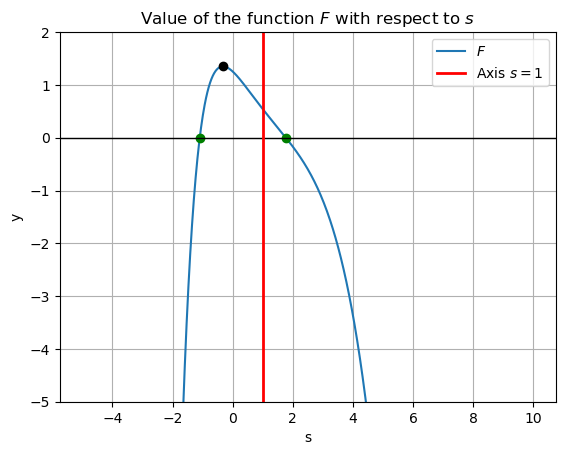
\includegraphics[scale=0.4]{pictures/F_sum_eps.png}
    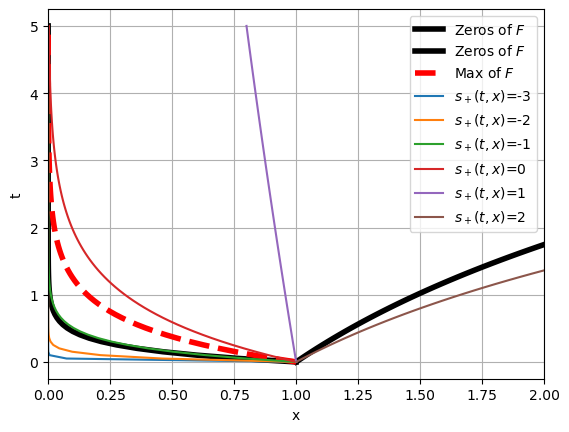
\includegraphics[scale=0.4]{pictures/paths_sum_eps.png}
    \caption{\textbf{Left:}
    Function $F(s)$ for $k_0 =  \frac12 \delta_{1-\varepsilon} + \frac12 \delta_{1 + \varepsilon}$. We see there are two zeros. \textbf{Right:} Several curves of the form $s_+ = \gamma$ for different values of $\gamma$. Between the black curves, $u(t,x)$ tends to infinity. Outside, $u(t,x)$ tends to zero exponentially fast. The red dotted line correspond to the curve where $F$ achieves a global maximum.}
    \label{fig:sum_eps}
    \end{figure} \\

    \textbf{Example 2: The uniform kernel $k_0 =  \1{[0.1; 1.1]}$} \\
    For  the uniform kernel $k_0 =  \1{[0.1; 1.1]}$, we have $K(s) = \frac{1}{s}\cdot \frac{1.1^s-0.1^s}{1.1-0.1}$. Let $\mu = 0.7$. 
    We plot $F$ and several curves of the form $s_+ = \gamma$ in Figure~\ref{fig:unif_0.1_1.1} 
    \begin{figure}
    \centering
    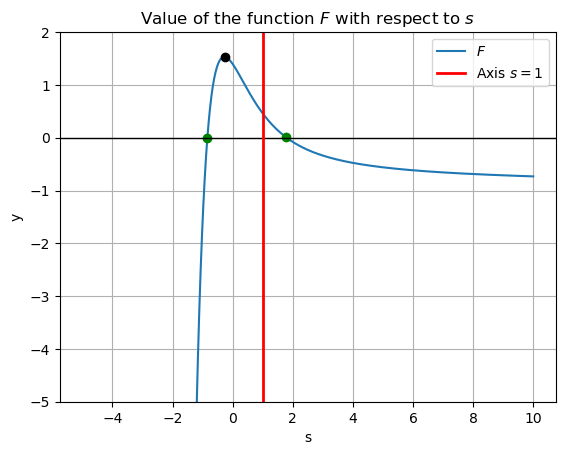
\includegraphics[scale=0.4]{pictures/F_unif_0.1_1.1.png}
    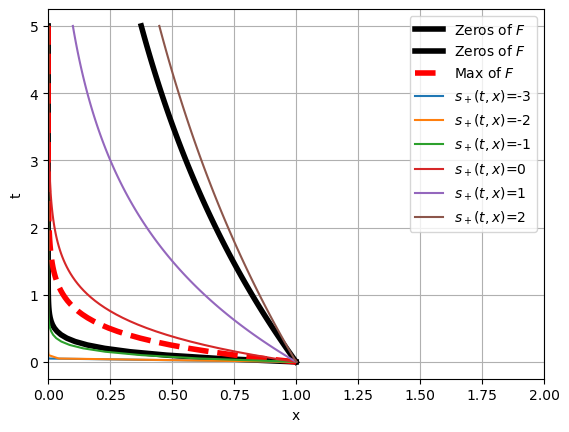
\includegraphics[scale=0.4]{pictures/paths_unif_0.1_1.1.png}
    \caption{\textbf{Left:}
    Function $F(s)$ for $k_0 =   \1{[0.1; 1.1]}$. We see there are two zeros. \textbf{Right:} Several curves of the form $s_+ = \gamma$ for different values of $\gamma$.  Between the black curves, $u(t,x)$ tends to infinity. Outside, $u(t,x)$ tends to zero exponentially fast. The red dotted line correspond to the curve where $F$ achieves a global maximum.}
    \label{fig:unif_0.1_1.1}
    \end{figure}\\

    \textbf{Example 3: The uniform kernel $k_0 =  \1{[0.98; 1.1]}$} \\
    For  the uniform kernel $k_0 =  \1{[0.98; 1.1]}$, we have $K(s) = \frac{1}{s}\cdot \frac{1.1^s-0.98^s}{1.1-0.98}$. Let $\mu = 0.7$. 
    We plot $F$ and several curves of the form $s_+ = \gamma$ in Figure~\ref{fig:unif_0.98_1.1}
    \begin{figure}
    \centering
    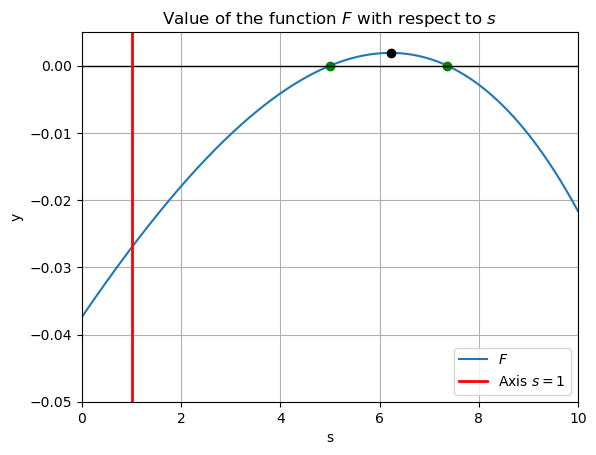
\includegraphics[scale=0.4]{pictures/F_unif_0.98_1.1.png}
    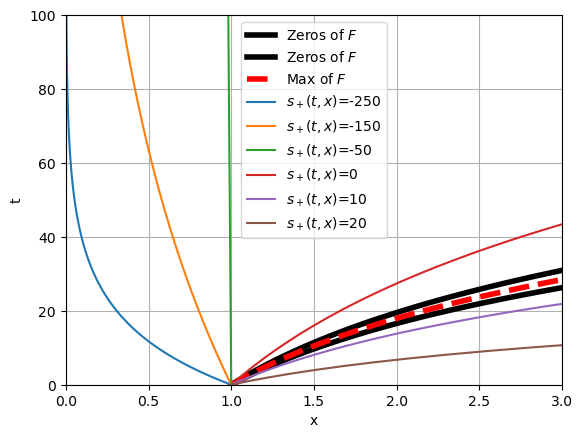
\includegraphics[scale=0.4]{pictures/paths_unif_0.98_1.1.png}
    \caption{\textbf{Left:}
    Function $F(s)$ for $k_0 =   \1{[0.98; 1.1]}$. We see there are two zeros. \textbf{Right:} Several curves of the form $s_+ = \gamma$ for different values of $\gamma$.  Between the black curves, $u(t,x)$ tends to infinity. Outside, $u(t,x)$ tends to zero exponentially fast. The red dotted line correspond to the curve where $F$ achieves a global maximum.}
    \label{fig:unif_0.98_1.1}
    \end{figure}\\

    \textbf{Example 4: The uniform kernel $k_0 =  \1{[0.1; 5]}$} \\
    For  the uniform kernel $k_0 =  \1{[0.1; 5]}$, we have $K(s) = \frac{1}{s}\cdot \frac{1.5^s-0.1^s}{1.5-0.1}$. Let $\mu = 0.7$. 
    We plot $F$ and several curves of the form $s_+ = \gamma$ in Figure~\ref{fig:unif_0.1_5}
    \begin{figure}
    \centering
    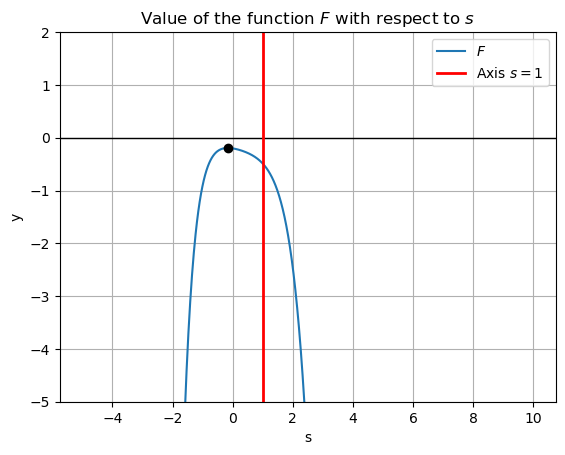
\includegraphics[scale=0.4]{pictures/F_unif_0.1_5.png}
    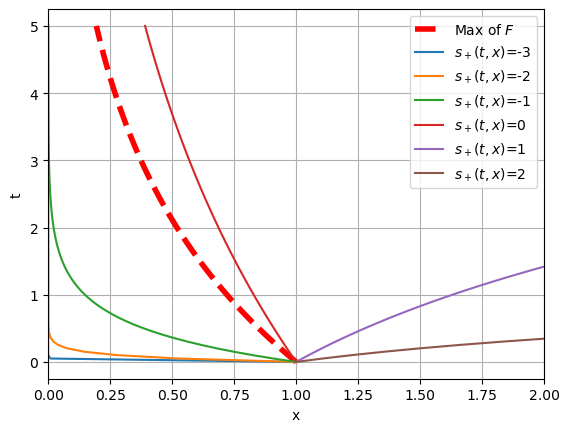
\includegraphics[scale=0.4]{pictures/paths_unif_0.1_5.png}
    \caption{\textbf{Left:}
    Function $F(s)$ for $k_0 =   \1{[0.1; 5]}$. We see there is no zero. \textbf{Right:} Differents curves of the form $s_+ = \gamma$ for different values of $\gamma$. The red dotted line correspond to the curve where $F$ achieves a global maximum. }
    \label{fig:unif_0.1_5}
    \end{figure}

% \section{Addition of a term of growth \ndr{Fusion avec le paragraph d'après}}

% Consider the equation
% \begin{equation*}
%     \begin{cases}
%         \frac{\partial}{\partial t}u(t,x) = - \mu u(t,x) + \mu \int\limits_{0}^{\infty}  k\big( \frac{x}{y}\big) u(t,y) \frac{\dy}{y} + xu(t,x)
%         & \text{for }t \in \RR_+, \; x \in \RR_+ \eqfinv
%         \\
%         u(0, x) = u_0(x)
%         & \text{for }x \in \RR_+
%         \eqfinp
%         \end{cases}
% \end{equation*}
% with $\mu \in (0, \infty)$. 

% By applying the Mellin transform, we have
% 	\begin{equation*}
% 		\frac{\partial}{\partial t} U(t,s) = - \mu U(t,s) + \mu K(s) U(t,s) + U(t,s+1)
% 		\eqfinp
% 	\end{equation*}
% It follows that
%     \begin{equation}
%         \frac{\partial}{\partial t} U(t,s) = - \mu (1-K(s)) U(t,s) + U(t,s+1)
% 		\eqfinp
%         \label{eq:addgrowth}
%     \end{equation}

% We consider the Laplace transform of $t \mapsto U(t,s)$
% $$ L(p,s) = \int_0^\infty U(t,s)e^{-pt}\diff t$$ 

% By applying the Laplace transform to Equation \eqref{eq:addgrowth} we have 
% \begin{align*}
%     pL(p,s) - U_0(s) = -  \mu (1-K(s)) L(p,s) + L(p,s+1)
% \end{align*}
% It follows that 
% \begin{align*}
%     L(p, s+1) = - U_0(s) + \big[\mu (1-K(s)) + p \big]L(p, s)
%     \eqfinp
% \end{align*}

% \begin{remark}
% We denote $\alpha(s) = \mu (1-K(s)) + p$. If $s \in \NN$, and if all quantities are well defined, we have that
% \begin{align*}
%     L(p, s+1) = -U_0(s) -\sum_{n = 1}^{s} \prod_{j = n}^s \alpha(s)U_0(s-1) + L(p,0) \prod_{n = 0}^{s}\alpha(n)
% \end{align*}
% \end{remark}



\section{Linear mutation rate}

In this section we {\MD consider a whole population dynamics, in a constant environment (infinite space and nutrient). Since $x$ represents the individual growth rate, it is well-known that $x$ is also the Malthus parameter of a clonal population which reproduces by fission and grows at this rate $x$~\cite{robert:hal-00981312}. Rather than a constant mutation rate, we now} assume that the number of mutations is proportional to the growth rate $x$. This modelling assumption can be justified by the fact that a mutation corresponds to an error in DNA replication %\cite{pray2008dna}. 
When a cell grows faster, it replicates its DNA faster. This increases the number of errors and therefore the number of mutations.\\

We {\MD thus} consider the following problem:
\begin{equation}
    \begin{cases}
	\frac{\partial}{\partial t}u(t,x) = x(1-\mu) u(t,x) + \mu \int\limits_{0}^{\infty} y k\big( \frac{x}{y}\big) u(t,y) \frac{\dy}{y} 
	& \text{for }t \in \RR_+, \; x \in \RR_+ \eqfinv
	\\
	u(0, x) = u_0(x)
	& \text{for }x \in \RR_+
	\eqfinp
    \end{cases}
    \label{eq:linearmutrate}
\end{equation}
Here, $u(t,x)$ represents the density of cells with a growth rate $x$ at the time $t$. The mutation rate is given by $\mu x$ with $\mu>0$ a given constant. \\

We consider several assumptions upon the mutation kernel.
\begin{hypothesis}\label{hyp:boundK} \mbox{}
    \begin{enumerate}
        \item We assume that $\mu < 1$ and that the fundamental strip of $K$ contains $[0, \infty)$.  
        %%\blue{Eventually, we may only assume that $K(s) \leq \frac{C}{s^k}$} 
        \item We suppose there exists {\MD $s_0\in \R,\;\ep_b>0$ such that on the} vertical strip $\{s \in \CC \;;\; \Re(s) \in(s_0-\varepsilon_b, s_0+1+\varepsilon_b) \},$ {\MD the Mellin transform $K$ of the kernel $k$ satisfies}
        $$|K(\Re(s))| < \frac{1}{\mu} - 1
        \mtext{for } \eqsepv s \in \CC \;\; s.t \;\; \Re(s) \in(s_0-\varepsilon_b, s_0+1+\varepsilon_b)\eqfinp$$ 
    \end{enumerate}
\end{hypothesis}
We note that the first assumption has a biological interpretation: we want the mutation {\MD rate} to be less than the natural growth {\MD rate, i.e., the average division rate}. The fact that the  fundamental strip of $K$ is $[0, \infty)$ means that $k_0$ decreases {\MD faster than any power law at $\infty$ and is such that $\int_0 x^{-1} k(\dd x) <\infty$, hence}
\begin{equation*}
    \begin{cases}
        k(x) = o\left( \frac{1}{x^s}\right) & \text{for every } s \in (1, \infty) \text{ when } x \to \infty \eqfinv\\
        k(x) = o\left( \frac{1}{x^s}\right) & \text{for every } s \in (0, 1) \text{ when } x \to 0 \eqfinp
    \end{cases}
\end{equation*}
The second assumption means that $\mu$ is small enough so that  such an interval exists. For instance if $\mu<\frac{1}{2}$ we have $K(1)=1<\frac{1}{\mu}-1$. The fact that $\mu$ is small means that mutations are (relatively) rare events. \\
%\ndr{: Détailler ++, rajouter une figure et discuter d'une valeur de $\mu^* $ critique}. 


To obtain a solution to Equation~\eqref{eq:linearmutrate}, our strategy is to transform it by successively applying a Mellin transform and then a Laplace transform. By complex analysis arguments, we can then obtain an explicit expression for the Laplace-Mellin transform, which we can invert and study in order to obtain asymptotic expansions for large times and small or large trait $x$. \\

By applying the Mellin transform in the $x$ variable, we have
    \begin{equation}
    \label{eq:addgrowtheasy}
	\begin{cases}
		\frac{\partial}{\partial t} U(t,s)
        = \left[- \mu (1-K(s)) + 1\right] U(t,s+1)
        & \text{for } t \in \RR_+, \; s \in S_M 
        \\
        U_0(s) 
        = \Mcal(u_0)(s) 
        & \text{for } s \in S_M 
		\eqfinv
	\end{cases}
    \end{equation}
where $S_M$ denotes the vertical strip where the Mellin transform of $u(t,\cdot)$ is defined and analytic. \\

We consider the Laplace transform of $t \mapsto U(t,s)$
\begin{align}
    L(z,s) = \int_0^\infty U(t,s)e^{-zt}\diff t
    \eqfinp
\end{align}

By applying the Laplace transform to Equation \eqref{eq:addgrowtheasy} in the $t$ variable we have 
\begin{align*}
    zL(z,s) - U_0(s) = \left[- \mu (1-K(s)) + 1\right] L(z,s+1)
\end{align*}
It follows that 
\begin{equation}
\begin{aligned}
    \label{eq:wienerhopfeq}
    zL(z,s) 
    &= \left[- \mu (1-K(s)) + 1\right] L(z, s+1) + U_0(s) \\
    &= \Phi(s) L(z, s+1) + U_0(s)
    \eqfinv
\end{aligned} 
\end{equation}
where $\Phi(s) \coloneqq \left[- \mu (1-K(s)) + 1\right]$. \\

{\MD We see that~\eqref{eq:wienerhopfeq} links $L(z,s)$ on the left-hand side to $L(z,s+1)$ on the right-hand side.  Such equation can be solved using} the Wiener--Hopf method,  successfully implemented e.g. in~\cite{escobedo2007fundamental} to solve the linearized Uehling-Uhlenbeck equation. For a general description of this method the reader may consult the Chapter 4 of \cite{zakharov2012kolmogorov}. 
\medskip

%The aim is to find for any $z \in \CC$ such that $\Re(z) > 0$ a solution  $L(z, \cdot)$ of~\eqref{eq:wienerhopfeq} which is analytic in the strip $S = \{\xi \in \CC \mid \Re(\xi) \in (s_0, s_0+1)\}$. The analyticity of $L(z, \cdot)$ strongly depends on the analytic properties of $K$. 

We present briefly the different steps of the Wiener--Hopf method. 

\begin{itemize}
    \item \textit{Step 1 - Change of variables:} We transform by a change of variable Equation~\eqref{eq:wienerhopfeq}, {\MD which links the solution $L(z,\cdot)$ to $L(z,\cdot +1)$,  where $L$ is defined on a strip $(a,b)+i\RR,$} into an equation {\MD which links $g(z,x+i0)$ to $g(z,x-i0)$} {\MD  where the unknown is} the function $g : \CC \setminus \RR_+ \to \CC$  
     (See Figure~\ref{f:WH}).
    On the line $\RR_+$, $g(z,\cdot)$ satisfies the equation
    \begin{align*}
        z g(z, x+i0) = \varphi(x)g(z, x-i0) + 1 \, \qquad \text{for all $x\in\RR_+$}\eqfinv
    \end{align*}
    with 
    \begin{align*}
        g(z, x+i0) &= \lim_{\varepsilon\to 0^+}  g(z, xe^{i\varepsilon}),\\
        g(z, x-i0) &= \lim_{\varepsilon\to 0^+}  g(z, xe^{i(2\pi-\varepsilon)})\eqfinp 
    \end{align*}
    \begin{figure}
        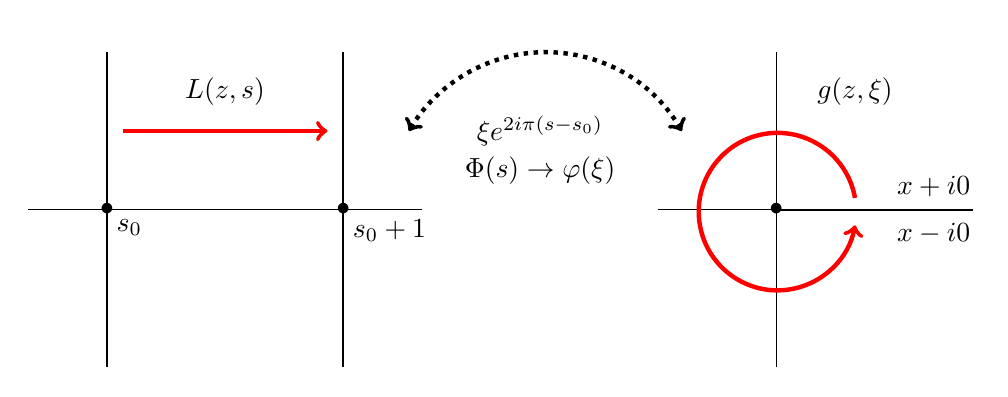
\begin{tikzpicture}
            \draw (1,0) node{$\bullet$} ;
            \draw (1,0) node[below right]{$s_0$} ;
            \draw (4,0) node {$\bullet$} ;
            \draw (4,0) node[below right]{$s_0+1$} ;
            \draw (0,0) -- (5, 0) ; % Trace le segment
            \draw[thick] (1,-2) -- (1, 2) ; % Trace le segment
            \draw[thick] (4,-2) -- (4, 2) ; % Trace le segment
            \draw (2.5,1.5) node{$L(z,s)$} ;
            \draw[-to, ultra thick, red] (1.2,1) -- (3.8, 1) ; % Trace la flêche
            \draw[to-to, ultra thick, dotted] (8.3,1) arc (30:150:2);
            \draw (6.5,1) node{$\xi \coloneqq e^{2i\pi(s-s_0)}$};
            \draw (6.5,0.5) node{$\Phi(s) \to \varphi(\xi)$};
            \draw (8,0) -- (12, 0) ;
            \draw (9.5,-2) -- (9.5, 2) ;
            \draw (10.5,1.5) node{$g(z, \xi)$} ;
            \draw (11.5,0.3) node{$x+i0$} ;
            \draw (11.5,-0.3) node{$x-i0$} ;
            \draw[-to, ultra thick, red] (10.5, 0.15) arc (10:350:1);
            \draw[thick] (9.5,0) -- (12, 0);
            \draw (9.5,0) node{$\bullet$};
            \end{tikzpicture}
        \label{f:WH}
        \caption{Illustration of the change of variables. The strip $\Re(s) \in (s_0, s_0+1)$ on the left is transformed in $\CC \setminus \RR_+$.  Red arrows show the \textit{"direction"} of the transformation. The line $s_0 + i\RR$ is transformed into $\RR_++i0$ and  $s_0 - i\RR$ is transformed into $\RR_+-i0$.}
    \end{figure}
    \item \textit{Step 2 - Find the good expression:} We aim to obtain an expression on $\CC \setminus \RR_+$ of the form 
    $ \Xi(z,x+i0) = \Xi(z,x-i0) $
    where $g$ is contained in the expression of $\Xi$. The goal is to obtain an expression that only depends on $x+i0$ (resp. $x-i0$) on the left (resp. right) side of the equality. This allows us to extend $\Xi$ on $\CC^*$ as an analytic function. 
     To obtain this expression, the key point is the Sokhotski--Plemelj formula \cite{sokhotski1873definite} that split a continuous function $f$ into two part {\MD \tt pas clair pour moi} $$f(x) = f_-(x-i0) + f_+(x+i0) \mtext{for} x \in (0,\infty)\eqfinp$$
    In the proof of Theorem~\ref{th:SolutionWH} below, we obtain the expression $$\Xi(\cdot) = M(z,\cdot)g(z, \cdot) -W(z,\cdot)$$  where $M$ and $W$ will be defined later. 
    \item \textit{Step 3 - The majoration:} In this part, we obtain bounds on $M$, $W$ and $g$ that compose the expression of $\Xi$. This allows us to apply Liouville's theorem to show that $\Xi$ is constant on $\CC^*$. {\MD From this, we obtain an}  explicit formula 
    $$ g = \frac{\Xi - W}{M} \eqfinp,$$
    \item \textit{Step 4 - Inversion of the transformation:} We revert the change of variables of Step 1 to obtain an explicit expression of $L(s,z)$ {\MD from the explicit expression of $g$}.    
\end{itemize}

In addition, the proof of Theorem~\ref{th:SolutionWH} is based on the following technical lemma which is proved in \cite{escobedo2007fundamental}.  
\begin{lemma}[Lemma C.2. in \cite{escobedo2007fundamental}]
    \label{escoARMA:C.2.}
    Suppose that $f$ is analytic in the cone 
    $$ C(2\varepsilon_0) \eqqcolon \{ \zeta \in \CC \,;\,\ \zeta = |\zeta|e^{i\theta}, \theta \in (-2\varepsilon_0, 2\varepsilon_0)\}$$
    for some $\varepsilon_0 > 0$. Let us also assume that 
    \begin{align}
        \label{escoARMA:C5} \int_0^\infty \frac{|f(re^{i \theta})|}{1+r^2} \diff r < \infty \mtext{for any} \theta \in (-2\varepsilon_0, 2\varepsilon_0) \\
        \label{escoARMA:C6} \lim_{\lambda \to 0 \,,\, \lambda \in C(2\varepsilon_0)} f(\lambda) = L_1 
        \eqsepv \lim_{\lambda \to \infty \,,\, \lambda \in C(2\varepsilon_0)} f(\lambda) = L_2 \\
        \label{escoARMA:C7} |f'(\lambda)| = o(\frac1\lambda) \mtext{as} \lambda \to 0 \,,\,\lambda \to \infty \,,\, \lambda \in C(2\varepsilon_0). 
    \end{align}
    Then, for any $\lambda_0 \in \CC \setminus C(2\varepsilon_0)$, the function
    \begin{align}
        \label{escoARMA:C8} F(\zeta) = \frac{1}{2i\pi} \int_0^\infty f(\lambda) \left( \frac{1}{\lambda - \zeta} - \frac{1}{\lambda - \lambda_0}\right) \diff \lambda
    \end{align} 
    is well-defined and analytic in the domain $D(\varepsilon_0) \subset S$. Moreover
    \begin{align}
        F(\zeta) &= - \frac{L_1}{2i\pi} \ln(\zeta) + o(\ln |\zeta|) \mtext{as} \zeta \to 0 \eqsepv \zeta \in D(\varepsilon_0) \\
        F(\zeta) &= - \frac{L_2}{2i\pi} \ln(\zeta) + o(\ln |\zeta|) \mtext{as} \zeta \to \infty \eqsepv \zeta \in D(\varepsilon_0)
    \end{align} 
\end{lemma}

\subsection{Resolution of the equation}

\begin{theorem}
\label{th:SolutionWH}Consider Assumption~\ref{hyp:boundK}. 
For any $z \in \CC \setminus \RR_-$, we denote
\begin{equation}
    V(s) \coloneqq \exp \left[
        - \int\limits_{s_0-i\infty}^{s_0+i\infty}\log \left( \frac{\Phi(\sigma)}{1-\mu}\right)
        \cdot \left(
            \frac{1}{1-e^{2i\pi(s-\sigma)}} - \frac{1}{1-e^{2i\pi(\sigma_0-\sigma)}}
         \right) \diff \sigma 
        \right]
        \label{def:V}
    \end{equation}
and 
\begin{equation}\label{eq:exprL}
    L(z,s) 
    = 
   - \frac{1}{z}\int_{s_0-i\infty}^{s_0+i\infty} \frac{V(y)}{V(s)} e^{ \alpha(z)(y-s)}
   \frac{\diff y}{(e^{2i\pi(y-s)}-1)}
   \eqfinv
\end{equation}
with $\alpha(z) \coloneqq  
    \left(\log \left( \frac{z}{1-\mu}\right)\right)$.
Then $L(z,\cdot)$ is the unique solution of Equation~\eqref{eq:wienerhopfeq}
\end{theorem}

\subsubsection{Reformulating the equation}
\label{s:reformulate_eq}
\mbox{}

The first step is to transform Equation~\eqref{eq:wienerhopfeq} on a strip $[s_0, s_0+1] + i \RR$ into an equation on $\CC \setminus \RR_+$. For this, we introduce the variables:
    \begin{align}
        \zeta & \coloneqq T(s) \coloneqq e^{2i\pi(s-s_0)}, \label{def:zeta}\\
        g(z,\zeta) &\coloneqq L(z,s), \label{def:g} \\
        \varphi(\zeta) &\coloneqq \Phi(s) \eqfinp
        \label{def:Phi}
    \end{align}
Notice that the transformation $T$ transforms the complex plane $\CC$ in the Riemann surface association to the logarithmic function that we denote from now on as $\Scal$. The function $\varphi$ is meromorphic in this Riemann surface. We can characterize uniquely each of the sheets of this Riemann surface by means of the argument $\theta$ of $\zeta$, where $\zeta \coloneqq re^{i\theta}$. \\
We denote $D$ the following portion of the Riemann surface $\Scal$:
\begin{equation}\label{def:D}
D \coloneqq \{ \zeta \in \Scal \mid \zeta = re^{i\theta}, r > 0, 0 < \theta < 2\pi \}.
\end{equation}
Here, we consider the equation for the fundamental solution, \ie 
$$u_0(x) = \delta_1(x) \mtext{and} U_0(x) = 1 \eqfinv$$
with $U_0(s) = \Mcal(u_0)(s)$. 
Equation~\eqref{eq:wienerhopfeq} becomes
\begin{align}
    \label{eq:WH3.5}
    z g(z, x+i0) = \varphi(x)g(z, x-i0) + 1 \, \qquad \text{for all $x\in\RR_+$}
\end{align}
where, for any $x \in \RR_+$, 
\begin{align*}
    g(z, x+i0) &\eqqcolon \lim_{\varepsilon\to 0^+}  g(z, xe^{i\varepsilon}),\\
    g(z, x-i0) &\eqqcolon \lim_{\varepsilon\to 0^+}  g(z, xe^{i(2\pi-\varepsilon)}),\\
    %%\varphi(x) &\eqqcolon \lim_{\varepsilon\to 0^+}\tilde \varphi(xe^{i\varepsilon}) 
\end{align*}
\begin{proposition}
\label{p:explicit_g}
Under Assumption~\ref{hyp:boundK}, the function $g(z, \cdot)$ is analytic on $D$ defined by~\eqref{def:D} for any $z \in \CC \setminus \RR_-$ and
\begin{align*}
    g(z,\zeta) 
    &= 
    \frac{\zeta}{2i\pi z}\int_0^\infty  \frac{M(z,\lambda+i0)}{M(z,\zeta)} \frac{\diff \lambda}{\lambda(\lambda-\zeta)} \\
\end{align*}
where $\lambda_0 \in \CC \setminus \RR_+$ and 
$$ M(z, \zeta) \coloneqq \exp\left(-{\frac{1}{2i\pi  }\int_0^\infty \ln\left(\frac{\varphi(\lambda)}{z}\right) \left( \frac{1}{\lambda-\zeta} - \frac{1}{\lambda-\lambda_0}\right) \diff \lambda} \eqfinp\right)$$ 
\end{proposition}
\begin{proof}
For any $s \in \RR_+$, $K(s) > 0 > 1 - \frac1\mu$. Then, 
for all $\zeta \in \RR_+^*$, $\varphi(\zeta) > 0$.
Since $\varphi$ is analytic on $\CC$, it follows that for all $x \in \RR_+$ 
    $$\varphi(x) 
    = \lim_{\varepsilon \to 0^+} \varphi(xe^{i\varepsilon}) 
    = \lim_{\varepsilon \to 0^-}\varphi(xe^{-i\varepsilon}) 
    = \varphi(x) > 0 \eqfinp$$
For any complex number $r = |r|e^{i\theta}$ we define the following branch of the complex logarithm
\begin{equation}\label{def:log}
\ln(r) \coloneqq \ln(|r|) + i\theta \eqsepv -\frac{\pi}{4} \leq \theta < 2\pi - \frac{\pi}{4}  \eqfinp
\end{equation}
Let us denote for $\zeta \in D \subset \Scal$
    \begin{align}\label{def:H}
        H(z,\zeta) \coloneqq \frac{1}{2i\pi }\int_0^\infty \ln\left(\frac{\varphi(\lambda)}{z}\right) \left( \frac{1}{\lambda-\zeta} - \frac{1}{\lambda-\lambda_0}\right) \diff \lambda
    \end{align}
for a given $\lambda_0 \in D$ and $z \in \CC \setminus \RR_-$. We notice that for $\lambda \in (0,\infty)$ we have $\varphi(\lambda)=1-\mu(1-K(s_0-\f{i}{2\pi} \ln(\lambda))$.\\

There are three things to verify that $H$ is well-defined for $\zeta \in D$. 
\begin{itemize}
    \item (Step 1) The integrand is integrable in $0$
    \item (Step 2) The integrand is integrable in $\infty$
    \item  (Step 3) The quantity $\ln\left(\frac{\varphi(\lambda)}{z} \right)$ is bounded on $(0, \infty)$.
\end{itemize}
\textit{Step 1: Existence when $\lambda \to 0$:}\\
We have that: 
\begin{align*}
    \lim_{\lambda \to 0}\frac{\varphi(\lambda)}{z} = \lim_{\nu\to-\infty}\frac{-\mu(1-K(s_0+i\nu))+1}{z} = \frac{-\mu+1}{z}
    \eqfinp
\end{align*}
\textit{Step 2: Existence when $\lambda \to \infty$:}
\begin{align*}
    \lim_{\lambda \to \infty}\frac{\varphi(\lambda)}{z} = \lim_{\nu\to\infty}\frac{-\mu(1-K(s_0+i\nu))+1}{z} = \frac{-\mu+1}{z}
    \eqfinp
\end{align*}
\textit{Step 3: We shot that for all $\lambda \in \RR$, $|\varphi(\lambda)| > \varepsilon$: }\\
For any $s \in s_0 + i\RR$, we have
    \begin{align*}
        |-\mu(1-K(s))+1| 
        = \mu \left|K(s) - \left(1-\frac{1}{\mu}\right)\right|
        \eqfinp
    \end{align*}
By Assumption~\ref{hyp:boundK}, for any $s \in s_0 + i\RR$, $|K(s)| \leq K(s_0) < \frac{1}{\mu} - 1$. It follows that
\begin{align*}
    \forall s \in s_0 + i\RR
    \eqsepv
    \left|K(s) - \left(1-\frac{1}{\mu}\right)\right| \geq \frac{1}\mu - 1 - K(s_0) > 0
    \eqfinp
\end{align*}
It follows that $\lambda \mapsto \ln\Big(\frac{\varphi(\lambda)}{z}\Big)$ is bounded on $(0, \infty)$\\

Therefore
$H(z,\zeta)$ is well defined.\\

The formulae of Plemej Sojoltski \cite{sokhotski1873definite} ensure that for $x > 0$
    \begin{align*}
        H(z,x+i0) &= \frac{1}{2} \ln\left(\frac{\varphi(x)}{z}\right) + \frac{1}{2i\pi } PV\int_0^\infty \ln\left(\frac{\varphi(\lambda)}{z}\right) \left( \frac{1}{\lambda-\zeta} - \frac{1}{\lambda-\lambda_0}\right) \diff \lambda\\
        H(z,x-i0) &= -\frac{1}{2} \ln\left(\frac{\varphi(x)}{z}\right) + \frac{1}{2i\pi } PV\int_0^\infty \ln\left(\frac{\varphi(\lambda)}{z}\right)\left( \frac{1}{\lambda-\zeta} - \frac{1}{\lambda-\lambda_0}\right) \diff \lambda
    \end{align*}
where $PV$ denotes the principal value. 
By substracting these expressions and composing by the exponential, we obtain:
\begin{align}
    \label{eq:phi_over_z}
    \frac{\varphi(x)}{z}
    = \frac{e^{-H(z,x-i0)}}{e^{-H(z,x+i0)}} 
    = \frac{M(z,x-i0)}{M(z,x+i0)}.
\end{align}
where we have defined
\begin{equation}
    M(z,\zeta) = e^{-H(z,\zeta)}
    \mtext{for}
    \zeta \in D
    \eqsepv z \in \CC \setminus \RR_- \eqfinp
    \label{def:M}
\end{equation}
Equation \eqref{eq:WH3.5} gives
\begin{align*}
    g(z, x+i0) = \frac{\varphi(x)}{z} g(z, x-i0) + \frac{1}{z} \, \qquad \text{for all $x\in\RR_+^*$}
\end{align*}
so that together with \eqref{eq:phi_over_z} we have
\begin{align*}
    g(z, x+i0) = \frac{M(z,x-i0)}{M(z,x+i0)} g(z, x-i0) + \frac{1}{z} \, \qquad \text{for all $x\in\RR_+^*$}.
\end{align*}
Then 
\begin{align*}
    M(z,x+i0)g(z, x+i0) = M(z,x-i0)g(z, x-i0) + \frac{M(z,x+i0)}{\cte  z} \, \qquad \text{for all $x\in\RR_+^*$}.
\end{align*}

We define the function
\begin{align}\label{def:W}
    W(z, \zeta) = \frac{1}{2i\pi }\int_0^\infty  \frac{M(z,\lambda+i0)}{z}\left( \frac{1}{\lambda-\zeta} - \frac{1}{\lambda-\lambda_0}\right) \diff \lambda 
    \eqfinp
\end{align}
To verify if this function is well-defined, we study the asymptotic behaviour of $M$ when $\lambda \to 0$ and $\lambda \to \infty$. For this, we verify that the function $f(\zeta) = \ln(\frac{\varphi(\zeta)}{z})$ satisfies the hypothesis of the Lemma~\ref{escoARMA:C.2.}
\begin{enumerate}
\item We verify Hypothesis~\eqref{escoARMA:C5}: It's straightforward to prove that 
    $$\int_0^\infty \frac{|f(r e^{i\theta)}|}{1+r^2}\diff r < +\infty$$ because due to Assumption~\ref{hyp:boundK}, $f(re^{i\theta})$ is bounded for any $\theta \in (-2\varepsilon_0, 2\varepsilon_0)$ when $\frac{2\varepsilon_0}{2\pi} < \varepsilon_b$. 
    \item We verify Hypothesis~\eqref{escoARMA:C6}: The Riemann-Lebesgue lemma ensures that 
    $$ \lim_{\lambda \to 0, \lambda \in C(2\varepsilon_0)} f(\lambda) = 
     \lim_{\lambda \to \infty, \lambda \in C(2\varepsilon_0)} f(\lambda)=\ln(\frac{1-\mu}{z}) 
 \eqqcolon L\eqfinp$$
    \item We verify Hypothesis~\eqref{escoARMA:C7}: Denoting $\lambda = e^{2i\pi(s-s_0)}$, we have that $\frac{\diff \lambda}{\diff s} = 2i\pi e^{2i\pi(s-s_0)} = 2i\pi \lambda$. Then 
    $\frac{\diff s}{\diff \lambda} = \frac{1}{2i\pi\lambda}$. 
    If follows that 
    $$f'(\lambda) = \frac{\varphi'(\lambda)}{\varphi(\lambda)} = \frac{\mu K'(s)}{1 - \mu + \mu K(s)}\frac{\diff s}{\diff \lambda} = \frac{\mu K'(s)}{1 - \mu + \mu K(s)} \cdot \frac{1}{2i\pi\lambda}. $$
    If $\lambda \to 0$, then $s \to s_0+i\infty$ and If $\lambda \to \infty$, then $s \to s_0-i\infty$.  By the Riemann-Lebesgue lemma, it follows in both cases that $$K'(s) \to 0 \mtext{and} K(s) \to 0$$ then  $|\lambda f'(\lambda)| \to 0$ which ensure that $|f'(\lambda)| = o(\frac{1}{\lambda})$. \\
\end{enumerate}
Therefore, we can apply the Lemma~\ref{escoARMA:C.2.} which gives the next lemma. 

\begin{lemma}\label{EscARMA:C2}For any $\lambda \in \CC \setminus C(2\varepsilon_0)$, the function $H(z,\zeta)$ is analytic in the domain $D(\varepsilon_0) = \{ \zeta \in \Scal; \, \zeta = |\zeta|e^{i\theta}, \, \theta \in (-\varepsilon_0, 2\pi+\varepsilon_0)\}$ and 
$$ H(z, \zeta) = -\frac{L}{2i\pi } \ln(\zeta) + o(\ln(|\zeta|)) \mtext{as} \zeta\to 0,\, \zeta \in D(\varepsilon_0)$$ 
$$ H(z, \zeta) = -\frac{L}{2i\pi } \ln(\zeta) + o(\ln(|\zeta|)) \mtext{as} \zeta\to \infty,\, \zeta \in D(\varepsilon_0)$$ 
with $L = \ln(\frac{1-\mu}{z})$. 
\end{lemma}

By Definition, $ M(z, \zeta) = \exp(-H(z, \zeta))$. This function is analytic on the domain $D$. Lemma~\ref{EscARMA:C2} ensures that

\begin{lemma}\label{prop:cptM}The function $\zeta \mapsto M(z,\zeta)$ that was defined and analytic for $\zeta \in D$ has an analytic extension to the domain $D(\varepsilon_0)$ for $\varepsilon_0$ small enough. Moreover, for any $\varepsilon > 0$, there exist $\delta \in {\MD (-\f{1}{2}-\ep,\f{1}{2}+\ep)}$ such that, for any $z$ in the region
    $$ \Zcal_\varepsilon \coloneqq \{ z \in \CC :\, \arg z \in {\MD (-\pi-\varepsilon, \pi +\varepsilon)}\} \eqfinv$$ we have that 
    \begin{equation}
        |M(z, \zeta)| + |\zeta|\left| \frac{\partial}{\partial \zeta}M(z,\zeta)\right|
        \leq 
        C(z) |\zeta|^\delta \mtext{for} |\zeta| < 2 \eqsepv \zeta \in D(\varepsilon_0)
    \end{equation}
    and 
    \begin{equation}
        |M(z,\zeta)| \leq C(z)|\zeta|^{\delta} \mtext{for} |\zeta| > 2 \eqsepv \zeta \in D(\varepsilon_0)
    \end{equation}
\end{lemma}
\begin{proof}We follow the demonstration of Lemma C1 in \cite{escobedo2007fundamental}. From Lemma~\ref{EscARMA:C2} and from the fact that $M(z, \zeta) = \exp(-H(z,\zeta))$ it follows that $M$ has an analytic extension on $D(\varepsilon_0)$.
As $\zeta \to 0$, Lemma~\ref{EscARMA:C2} ensures that 
$$ M(z, \zeta) = \exp\left(\frac{L}{2i\pi } \ln(\zeta) + o(\ln(|\zeta|)) \right)  \mtext{as} \zeta\to 0,\, \zeta \in D(\varepsilon_0) \eqfinp$$
hence
$$ \vert {M(z,\zeta)}{} \vert \leq {\MD Cst} \vert {|\zeta|^{\frac{L}{2i\pi}}}\vert=
\vert |\zeta|^{\frac{\log(\frac{1-\mu}{z})}{2i\pi}}\vert = \vert \zeta \vert^{\frac{\arg (\frac{1-\mu}{z})}{2\pi}}=\vert \zeta \vert^\delta
\mtext{for}  \vert \zeta \vert < 1,\, \zeta \in D(\varepsilon_0)$$ with 
 $\delta = \frac{\arg(\frac{1}{z})}{2\pi}$. We note that {\MD $\delta \in (-\f{1}{2}-\f{\ep}{2\pi},\f{1}{2}+\f{\ep}{2\pi})$ because $\arg(\frac{1}{z}) \in (-\pi-\ep, \pi+\ep)$}.
Since $M(z, \cdot)$ is analytic, the Cauchy estimates ensure that 
\begin{equation*}
    |M(z, \zeta)| + |\zeta|\left| \frac{\partial}{\partial \zeta}M(z,\zeta)\right|
    \leq 
    C(z) |\zeta|^\delta \mtext{for} |\zeta| < 2 \eqsepv \zeta \in D(\varepsilon_0)
\end{equation*}

Similarly, as $\zeta \to \infty$, Lemma~\ref{EscARMA:C2} ensures that 
\begin{align*}
    |M(z, \zeta)| 
    = 
    \exp\left(\frac{L}{2i\pi } \ln(\zeta) + o(\ln(|\zeta|)) \right)  \mtext{as} \zeta\to \infty,\, \zeta \in D(\varepsilon_0),
\end{align*}
which implies 
$$ \vert {M(z,\zeta)}{} \vert \leq {\MD Cst }\vert {|\zeta|^{\frac{L}{2i\pi}}}\vert=
\vert |\zeta|^{\frac{\log(\frac{1-\mu}{z})}{2i\pi}}\vert = \vert \zeta \vert^{\frac{\arg (\frac{1-\mu}{z})}{2\pi}}=\vert \zeta \vert^\delta
\mtext{for}  \vert \zeta \vert > 1,\, \zeta \in D(\varepsilon_0)$$
\end{proof}

\begin{lemma}\label{lm:cptW}For any $z \in \Zcal_\varepsilon$, the function $W(z, \cdot)$ defined in~\eqref{def:W} is analytic on $D$ and there is $\delta \in (0,1)$ and a constant $C(z)$ such that
    $$ |W(z, \zeta)| \leq C(z) 
    \mtext{when} |\zeta| < 1 \eqsepv \zeta \in D$$
    and 
    $$ |W(z, \zeta)| \leq C(z)|\zeta|^\delta \mtext{when} |\zeta| > 1 \eqsepv \zeta \in D$$
\end{lemma}
%cela suit la preuve du lemme C3 ARMA
\begin{proof}Lemma~\ref{prop:cptM} ensures that $W(z,\cdot)$ is well defined and analytic on $D$.\\

\textit{(1st case): }For any $\zeta \in D$ such that $|\zeta| < \frac{1}{2}$, 
\begin{align*}
    W(z, \zeta) = \int_0^{2|\zeta|} (\ldots)\diff \lambda + \int_{2|\zeta|}^1 (\ldots) \diff \lambda + \int_1^\infty (\ldots) \diff \lambda \coloneqq W_1 + W_2 + W_3 \eqfinp
\end{align*}
We have from Lemma~\ref{prop:cptM} that
    $$ |W_3| \leq C(z) \int_1^\infty \lambda^\delta \frac{1+|\lambda_0|}{|\lambda||\lambda - \lambda_0|} \diff \lambda < \infty \eqfinp$$
Since $\zeta \in D$, there is $\varepsilon_0 > 0$ such that $\arg \zeta \in (\varepsilon_0, 2\pi - \varepsilon_0)$. If $\lambda \in (0, 2|\zeta|)$, then $|\lambda-\zeta| \geq \frac{\varepsilon_0}{2}|\zeta|$. It follows that 
    $$ W_1 \leq C(z)\int_0^{2|\zeta|} \lambda^\delta \left(\frac{1}{(\lambda-\lambda_0)}+ \frac{2}{\varepsilon_0 |\zeta|}\right) \leq \frac{C(z)}{|\zeta|} \int_0^{2|\zeta|} \lambda^\delta \diff \lambda \leq C(z)|\zeta|^\delta \eqfinp$$
Similarly, we can prove that $|W_2| < \infty$ by using the fact that for all $\lambda \in (2|\zeta|, 1)$ $$|\lambda-\zeta|\geq\frac{|\lambda|}{2}.$$

\textit{(2nd case):} For any $\zeta \in D$ such that $|\zeta| > \frac{1}{2}$, 
\begin{align*}
    W(z, \zeta) = \int_0^{1} (\ldots)\diff \lambda + \int_1^\infty (\ldots) \diff \lambda \eqfinp
\end{align*} 
For all $\lambda \in (0,1)$, \\
For all $\lambda \in (1, \infty)$, 
   $$\left| \int_1^\infty (\ldots) \diff \lambda \right|
   \leq C \int_1^\infty |\lambda|^\delta \frac{|\zeta|} {|\lambda|\cdot|\lambda-\zeta|} \diff \lambda  
   = C \int_1^\infty |\lambda|^\delta \frac{1} {|\lambda|\cdot|\frac{\lambda}{|\zeta|}-1|} \diff \lambda \eqfinp$$
The change of variables $\lambda = x \zeta$ ensures that 
    $$ 
    \left| \int_1^\infty (\ldots) \diff \lambda \right|
    \leq 
    C \int_1^\infty |x|^\delta |\zeta|^\delta \frac{1} {|\zeta||x|\cdot|x-1|} |\zeta|\diff x \eqfinp
    \leq 
    C |\zeta|^\delta \int_1^\infty |x|^\delta \frac{1}{|x|\cdot|x-1|}\diff x \eqfinp
    \leq C |\zeta|^\delta
    $$
\end{proof}

The Sokhotski--Plemelj formula ensures that 
\begin{align*}
    \frac{M(z,x+i0)}{z}
    = 
    W(z,x+i0) - W(z,x-i0)
    \mtext{for any}
    x > 0
    \eqfinp
\end{align*}
Therefore, for all $x\in\RR_+$, 
\begin{align*}
    M(z,x+i0)g(z, x+i0) -W(z,x+i0) = M(z,x-i0)g(z, x-i0) - W(z,x-i0) \, \qquad \text{}.
\end{align*}
It follows that the function $C(z,\cdot)$ defined by 
$$ C(z,\cdot) \coloneqq M(z,\cdot)g(z,\cdot) - W(z,\cdot)$$
is analytic in $\CC \setminus \{0\}$.\\


Using the fact that $g$ is bounded on $\CC$, Lemma~\ref{prop:cptM} and Lemma~\ref{lm:cptW}
, the Liouville's theorem ensures that
\begin{align*}
    \forall z \in \CC \setminus \RR_-
    \eqsepv
    C(z,\zeta) = C(z)
\end{align*}
Then 
\begin{align}
    g(z,\zeta) = \frac{C(z)+W(z,\zeta)}{M(z,\zeta)}
\end{align}
However, Lemma~\ref{prop:cptM} and the boundeness of $g$ ensure that
\begin{align}
C(z) 
= \lim_{\zeta \to 0}[M(z,\cdot)g(z,\cdot) - W(z,\cdot)] 
= -\lim_{\zeta \to 0}W(z,\zeta)
\end{align}
As
$$ \lim_{\zeta \to 0}W(z,\zeta) 
= \frac{1}{2i\pi z}\int_0^\infty  {M(z,\lambda+i0)}\left( \frac{1}{\lambda} - \frac{1}{\lambda-\lambda_0}\right) \diff \lambda $$
we have that
\begin{align*}
    C(z) + W(z,\zeta)
    &= 
    \frac{1}{2i \pi z}\int_0^\infty  {M(z,\lambda+i0)}\left( \frac{1}{\lambda-\zeta}-\frac{1}{\lambda}\right) \diff \lambda \\
    &= 
    \frac{\zeta}{2i\pi z}\int_0^\infty  {M(z,\lambda+i0)}\frac{1}{\lambda(\lambda-\zeta)} \diff \lambda \\
\end{align*}
It follows that 
\begin{align}
    g(z,\zeta) 
    &\coloneqq 
    \frac{\zeta}{2i \pi z}\int_0^\infty  \frac{M(z,\lambda+i0)}{M(z,\zeta)} \frac{\diff \lambda}{\lambda(\lambda-\zeta)} \\
\end{align}
For any $z \in \CC \setminus \RR_-$, Equation~\eqref{def:M} ensures that $M(z, \cdot)$ does not vanish on $D$ and Lemma~\ref{prop:cptM} ensures that $M(z, \cdot)$ is analytic on $D(\varepsilon_0$). It follows that $g(z, \cdot)$ is analytic on $D$ for any $z \in \CC \setminus \RR_-$.

\end{proof}

\subsubsection{The solution of the Equation}
Now we want to return to the solution of Equation~\eqref{eq:wienerhopfeq}. For this purpose, we revert the change of variables \eqref{def:zeta},\eqref{def:g} and \eqref{def:Phi} which gives
\begin{align}
    L(z,s) = g(z, T(s)) \mtext{for all} z \in \CC \setminus \RR_+ \eqsepv s \in S 
    \eqfinp
\end{align}
We define $m(z,s) \coloneqq M(z, T(s))$. Then

\begin{align*}
    L(z,s) &= g(z,T(s)) \\ 
    &= 
    \frac{T(s)}{2i \pi z}\int_0^\infty  \frac{M(z,\lambda)}{m(z,s)} \frac{\diff \lambda}{\lambda(\lambda-T(s))} \\
    &= 
    \frac{1}{2i\pi z}\int_0^\infty  \frac{M(z,\lambda)}{m(z,s)} \frac{\diff \lambda}{\lambda\Big(\frac{\lambda}{T(s)}-1\Big)} \\
    &= 
    \frac{1}{2i\pi z}\int_0^\infty  \frac{M(z,\lambda)}{m(z,s)} \frac{\diff \lambda}{\lambda\Big(\frac{\lambda}{e^{2i\pi(s-s_0)}}-1\Big)} \\
\end{align*}
The change of variable $\lambda = e^{2i\pi(\sigma-s_0)}$ gives
\begin{align*}
    L(z,s)
    &= 
    - \frac{2i\pi }{2i\pi z}\int_{s_0-i\infty}^{s_0+i\infty}  \frac{m(z,\sigma)}{m(z,s)} \frac{\diff \sigma}{(e^{2i\pi(\sigma-s)}-1)} \\
    &= 
   - \int_{s_0-i\infty}^{s_0+i\infty} \frac{1}{z}  \frac{m(z,\sigma)}{m(z,s)} \frac{\diff \sigma}{(e^{2i\pi(\sigma-s)}-1)}. 
\end{align*}
The change of variable shows that
\begin{equation}
    m(z,s) = \exp \left[
    - \int_{s_0-i\infty}^{s_0+i\infty}\log \left( \frac{\Phi(
    \sigma)}{z}\right)
    \cdot \left(
        \frac{1}{1-e^{2i\pi(s-\sigma)}} - \frac{1}{1-e^{2i\pi(\sigma_0-\sigma)}}
     \right) \diff \sigma
    \right]
\end{equation} 
with $\lambda_0 = e^{2i\pi(\sigma_0 - s_0)}$. 
We have that 
\begin{equation}
    L(z,s) 
    = 
   - \int_{s_0-i\infty}^{s_0+i\infty} \frac{1}{z}  \frac{m(z,\sigma)}{m(z,s)} \frac{\diff \sigma}{(e^{2i\pi(\sigma-s)}-1)}
\end{equation}

We note that the term $\frac{m(z,\sigma)}{m(z,s)}$ depends on $z$.% For reasons that will become clearer later, we want to isolate this dependency in a term that can be calculated explicitly. 
We have
\begin{equation}
    m(z,s) = V(s)
    \exp \left[
    - \int\limits_{s_0-i\infty}^{s_0+i\infty} \left[\log \left( \frac{1-\mu}{z}\right)\right]
    \cdot \left(
        \frac{1}{1-e^{2i\pi(s-\sigma)}} - \frac{1}{1-e^{2i\pi(\sigma_0-\sigma)}}
     \right) \diff \sigma
    \right]
    \label{eq:uselogbranch}
\end{equation}
where 
\begin{equation}
V(s) \coloneqq \exp \left[
    - \int\limits_{s_0-i\infty}^{s_0+i\infty}\log \left( \frac{\Phi(\sigma)}{1-\mu}\right)
    \cdot \left(
        \frac{1}{1-e^{2i\pi(s-\sigma)}} - \frac{1}{1-e^{2i\pi(\sigma_0-\sigma)}}
     \right) \diff \sigma 
    \right]
    \eqfinp
\end{equation}

Then 
\begin{equation*}
    \frac{m(z,y)}{m(z,s)} 
    = 
    \frac{V(y)}{V(s)} \times E(z,y,s)
\end{equation*}
where $$E(z,y,s) \coloneqq \exp \left[
    - \int_{s_0-i\infty}^{s_0+i\infty} \left[\log \left( \frac{1-\mu}{z}\right) \right]
    \cdot \left(
        \frac{1}{1-e^{2i\pi(y-\sigma)}} - \frac{1}{1-e^{2i\pi(s-\sigma)}}
     \right) \diff \sigma \right]
     $$

We have that
\begin{equation*}
    E(z,y,s) 
    = 
    \exp
        \left[
     \left(\log \left( \frac{1-\mu}{z}\right) \right)
    \cdot (y-s)\right]
\end{equation*}

Then 
\begin{equation}
    \label{ARMA3.30}
    L(z,s) 
    = 
   - \frac{1}{z}\int_{s_0-i\infty}^{s_0+i\infty} \frac{V(y)}{V(s)} e^{ \alpha(z)(y-s)}
   \frac{\diff y}{(e^{2i\pi(y-s)}-1)}
\end{equation}
where $\alpha(z) \coloneqq  
    \left(\log \left( \frac{z}{1-\mu}\right)\right)$
\subsection{Asymptotic behaviour} In the previous section, we have established an explicit expression for $L(z,s)$. In this section, we want to obtain some information on the asymptotic behaviour of $u(t,x)$ that can be obtained by applying the inverse Laplace transform and the inverse Mellin transform to $L(z,s)$. \\

We recall that the inverse Mellin transform of $L(z,\cdot)$ is given by 
\begin{equation*}
    \tilde{L}(z,x) = \Mcal^{-1}(L(z, \cdot))[x] = \frac{1}{2i\pi} \int_{b-i\infty}^{b+i\infty} L(z,s)x^{-s}\diff s
    \eqsepv
    z \in \CC \setminus \RR_-
    \eqsepv x \in (0, \infty)
    \eqfinp
\end{equation*}
where $b$ is in $<s_0, s_0+1>$.\\
The inverse Laplace transform of $\tilde{L}(z,x)$ is given by 
\begin{equation*}
     \Lcal^{-1}(\tilde L(\cdot, x))[t] 
     = \frac{1}{2\pi i} \int_{c-i\infty}^{c+i\infty} e^{zt}\tilde L(z,x) \diff z
     \eqfinp
\end{equation*}
where $c \in \RR$ is large enough to have all the singularities of $\tilde L(\cdot,x)$ at the left of the line $\Re z = c$. 
\medskip

Since the function $L(z,s)$ is bounded, the operator $\Lcal^{-1}$ and $ \Mcal^{-1}$ are defined in the sense of tempered distribution \cite{misra1986transform}. It follows that the fundamental solution of the problem is given by 
    \begin{equation}
        u(t,x) = \Lcal^{-1} (\Mcal^{-1} (G))
        \eqfinp
    \end{equation}
    
In order the study the asymptotic behavior of $u(t,x)$ we need the following lemma: 
\begin{lemma}The function $V$ defined by Equation~\eqref{def:V} satisfies
    \begin{equation}
        V(s+1) = V(s)\frac{\Phi(s+1)}{1-\mu}
        \mtext{for}
        s \in (s_0, s_0+1) + i\RR
        \eqfinp
        \label{EscARMA:C4}
    \end{equation}
It can be extended meromorphically to $\CC$ using \eqref{EscARMA:C4}.
\end{lemma}
\begin{proof}
We follow the proof of Lemma~C4 in \cite{escobedo2007fundamental}
\end{proof}

\begin{remark}
    Equation~\eqref{EscARMA:C4} ensure that $V(s) = (1-\mu)\frac{V(s+1)}{\Phi(s+1)}$. 
    The function $V$ has no zero on the vertical strip $<s_0, s_0+1>$. Let $s_{pole} \in \CC$ be a pole of $\Phi$. Then $V$ has a zero for all $s \in \{s_{pole} - \NN^* \}$.
    Let $s_{zero} \in \CC$ be a zero of $\Phi$. Then $V$ has a zero for all 
    $s \in \{s_{zero} + \NN\}$. 
\end{remark}

Assumption: We suppose now that the function $\phi$ satisfies:
\begin{hypothesis}
    \label{ARMA_P3}
    We assume that the function $\Phi$ satisfies
    $$ |\Im \Phi(\xi) - \Im \Phi(\xi)_\infty| + |\xi|\cdot | \Im \Phi'(\xi) - \Im \Phi(\xi)_\infty| = \Ocal(|\xi|^{-\gamma-1}) $$
    with $\gamma > 0$, $\alpha > 0$ and 
    $$ \Phi(\xi)_\infty \coloneqq (1-\mu) + \frac{b_1}{\xi^\alpha} + \frac{b_2}{\xi} \eqfinp$$ 
\end{hypothesis}


    
\subsubsection{Description of $u(t,x)$ as $x \to \infty$}\text{\\}

From the definition of the inverse Mellin transform, we have
\begin{equation}
    \Mcal^{-1}[L(z,\cdot)](x) = \frac{1}{2i\pi} \int_{b-i\infty}^{b+i\infty} L(z,s)x^{-s}\diff s
    \eqsepv
    z \in \CC \setminus \RR_-
    \eqfinp
\end{equation}

The main contribution of $\Mcal^{-1}[L(z,\cdot)](x)$ as $x \to \infty$ is due to the closest pole $s_p$ of $L(z,\cdot)$ to the line $b+i\RR$ and right to this line. The pole of $L(z,\cdot)$ are given by the zeros of $V$. 

By deforming the contour integration to a line $d+i\RR$ with $d > \Re(s_p)$, The residue theorem ensures that
\begin{subequations}
\begin{align}
    \Mcal^{-1}[L(z,\cdot)](x) 
    &= - x^{-s_p}\res(L(z,\cdot);s = s_p) +  \frac{1}{2i\pi} \int_{d-i\infty}^{d+i\infty} L(z,s)x^{-s}\diff s\\
    &= - x^{-s_p}\res(L(z,\cdot);s = s_p) + o(x^{-\Re(s_p)})
    \eqfinp
\end{align}
\label{eq:exprMellinInv}
\end{subequations}
The residue of $L(z,\cdot)$ at the pole $s_p$ is given by 
\begin{equation*}
    \res(L(z,\cdot);s = s_p) 
    = 
    - \frac{1}{z}\res\left( \frac{1}{V(s)}; s = s_p\right) \int\limits_{s_0-i\infty}^{s_0+i\infty}
    V(\sigma) e^{ \alpha(z)(\sigma-s_p)}
   \frac{\diff \sigma}{(e^{2i\pi(\sigma-s_p)}-1)}
   \eqfinp
\end{equation*}
%\ndr{Just to recall even if there is no needs here : $\Re(\sigma-s_p) < 0$}

From Equation~\eqref{EscARMA:C4}, we obtain that
$$ V(s) = V(s-1)\frac{\Phi(s)}{1-\mu}
        \mtext{for}
        s \in (s_0+1, s_0+2) + i\RR
        \eqfinp$$
Then 
$$ \lim_{s\to s_p} \frac{V(s)}{s-s_p} 
= \lim_{s\to s_p} \frac{V(s-1)}{1-\mu} \frac{\Phi(s)-\Phi(s_p)}{s-s_p}
=  \frac{V(s_p-1)}{1-\mu} \Phi'(s_p) \neq 0 \eqfinp$$
%\ndr{It $\neq 0$ because $s_p$ is a simple pole... to be prove.}
Therefore, the  residue of $1/V$ at the pole $s = s_p$ is given by 
$$ \res\left( \frac{1}{V(s)}; s = s_p\right) = \frac{1-\mu}{V(s_p-1)} \frac{1}{\Phi'(s_p)} \eqfinp$$

\begin{equation}
    \res(L(z,\cdot);s = s_p) 
    = 
     \frac{-(1-\mu)}{z \Phi'(s_p) V(s_p-1)}
     \int\limits_{s_0-i\infty}^{s_0+i\infty}
    V(\sigma) e^{ \alpha(z)(\sigma-s_p)}
   \frac{\diff \sigma}{(e^{2i\pi(\sigma-s_p)}-1)}
   \eqfinp
\end{equation}

By using this expression in Equation~\eqref{eq:exprMellinInv}, we obtain that 
\begin{equation*}
    \Mcal^{-1}[L(z,\cdot)](x) 
    = x^{-s_p}\frac{1-\mu}{z \Phi'(s_p) V(s_p-1)}
     \int\limits_{s_0-i\infty}^{s_0+i\infty}
     \frac{V(\sigma) e^{ \alpha(z)(\sigma-s_p)}
  }{(e^{2i\pi(\sigma-s_p)}-1)}\diff \sigma + \frac{1}{2i\pi} \int_{d-i\infty}^{d+i\infty} L(z,s)x^{-s}\diff s
    \eqfinp
\end{equation*}

Taking the inverse Laplace transform, we obtain that: 
\begin{align*}
     u(t,x) &= \Lcal^{-1}(\tilde L(\cdot, x))[t] \\
     &= \frac{1}{2i\pi } \int_{c-i\infty}^{c+i\infty} e^{zt}\Mcal^{-1}[L(z,\cdot)](x) \diff z
     \eqfinp\\
     &= A(t)x^{-s_p} + B(t,x)
\end{align*}
with 
\begin{equation}
    A(t) \coloneqq\frac{1-\mu}{\Phi'(s_p) V(s_p-1)}
     \int\limits_{s_0-i\infty}^{s_0+i\infty}
     \frac{V(\sigma)
  }{(e^{2i\pi(\sigma-s_p)}-1)} \left[\int_{c-i\infty}^{c+i\infty} \frac{e^{ \alpha(z)(\sigma-s_p)}e^{tz}}{z}\diff z \right] \diff \sigma
  \label{def:A} 
\end{equation}
and 
\begin{equation}
    B(t,x) \coloneqq \frac{1}{2i\pi} \Lcal^{-1}\left[\int_{d-i\infty}^{d+i\infty} L(z,s)x^{-s}\diff s \right] (t)
\label{def:B}
\end{equation}

Let $\ln_{m}$ denote the main branch of the complex logarithm. There exists $k \in \ZZ$ such that for all $z \in \CC \setminus \{0\}$, $\ln_m(z) = \ln(z) + 2i\pi k. $ \\
We get that 
\begin{subequations}
\begin{align}
    \Lcal^{-1}\left[ \frac{e^{ \alpha(z)(\sigma-s_p)}}{z}  \right]
    &= 
    \Lcal^{-1}\left[ \frac{e^{ \left( \frac{\ln_m(z) + 2i\pi k}{1-\mu} \right) (\sigma-s_p)}}{z}  \right] \\
    &= 
    e^{ \left( \frac{2i\pi k}{1-\mu} \right) (\sigma-s_p)}
    \int_{c-i\infty}^{c+i\infty} e^{ \alpha(z)(\sigma-s_p)}e^{tz}\frac{\diff z}{z}\\
    &= \beta_p(\sigma) \Gamma(\sigma-s_p)((1-\mu)t)^{-(\sigma-s_p)}(e^{2i\pi(\sigma-s_p)}-1)
    \eqfinv
    \label{eq:4.24}
\end{align}
\label{eq:calcLaplInv}
\end{subequations}
where $\beta_p(\sigma) \coloneqq e^{ \left( \frac{2i\pi k}{1-\mu} \right) (\sigma-s_p)}$. 

The two next lemmas give estimates for $A$ and $B$. 

\begin{lemma}[An estimate for $A$] The following estimates hold: 
    \begin{align*}
        A(t) 
        &=  - \frac{t(1-\mu)^2}{\Phi'(s_p)} \res(\Gamma(z), z = -1) \\
        &+   \frac{1-\mu}{\Phi'(s_p) V(s_p-1)}
         \int\limits_{d-i\infty}^{d+i\infty}
         \beta_p(\sigma) V(\sigma)
       \Gamma(\sigma-s_p)\big((1-\mu)t\big)^{-(\sigma-s_p)} \diff \sigma \\
       &=  \frac{t(1-\mu)^2}{\Phi'(s_p)} + o(t)
      \eqfinp
    \end{align*}
    as $x \to \infty$ and $t \to \infty$.
\end{lemma}
\begin{proof}We get from Equations~\eqref{def:A} and \eqref{eq:calcLaplInv} that 
\begin{subequations}
    \begin{align}
    A(t) 
    &=
    \frac{1-\mu}{\Phi'(s_p) V(s_p-1)}
     \int\limits_{s_0-i\infty}^{s_0+i\infty}
     \frac{\beta_p(\sigma) V(\sigma)\Gamma(\sigma-s_p)
  }{(e^{2i\pi(\sigma-s_p)}-1)} \big((1-\mu)t\big)^{-(\sigma-s_p)}(e^{2i\pi(\sigma-s_p)}-1) \diff \sigma  \\
  &=  
   \frac{1-\mu}{\Phi'(s_p) V(s_p-1)}
     \int\limits_{s_0-i\infty}^{s_0+i\infty}
     \beta_p(\sigma) V(\sigma)
   \Gamma(\sigma-s_p)\big((1-\mu)t\big)^{-(\sigma-s_p)} \diff \sigma
  \eqfinp
\end{align}
\end{subequations}

We move the integration contour right to $\Re(\sigma) = s_0$. The pole of the function $\Gamma(\cdot-s_p)$ are located in $\{s_p - \NN\}$. Since $s_p$ is the first pole of $L(s,z)$ right to the vertical strip $<s_0, s_0+1>$, it follows that $s_p-1$ is first pole of $\Gamma(\cdot-s_p)$ right to the vertical line $\Re(\sigma) = s_0$. \\

Let $d \in (\Re(s_p)-1,\Re(s_p))$. The Residue Theorem ensures that 
\begin{align*}
    A(t) 
    &=  - \frac{t(1-\mu)^2}{\Phi'(s_p)} \res(\Gamma(z), z = -1) \\
    & +   \frac{1-\mu}{\Phi'(s_p) V(s_p-1)}
     \int\limits_{d-i\infty}^{d+i\infty}
     \beta_p(\sigma) V(\sigma)
   \Gamma(\sigma-s_p)\big((1-\mu)t\big)^{-(\sigma-s_p)} \diff \sigma \\
   &=  \frac{t(1-\mu)^2}{\Phi'(s_p)} + o(t)
  \eqfinp
\end{align*}
\end{proof}

\begin{lemma}[An estimate for $B$] The following estimates hold:
    \begin{align*}
        |B(t,x)| \leq  C e^{-\tilde b x} ((1-\mu)t)^{\tilde d - \tilde b} 
        & \text{ for } x > 1, \, 0 < t < 1 \eqfinp  \\
        |B(t,x)| \leq  C e^{-\tilde b x} ((1-\mu)t)^{r - \tilde b} 
        & \text{ for } x > 1, \, t \geq 1 \eqfinp 
    \end{align*}
    where $\tilde b < s_0$ is an arbitrary real number, $\tilde d > s_0 +1$ is an arbitrary real number and $r$ is an arbitrary number less than $s_p$. 
\end{lemma}
\begin{proof}
    Let us recall Equation~\eqref{def:B},  
    \begin{equation*}
        B(t,x) \coloneqq \frac{1}{2i\pi} \Lcal^{-1}\left[\int_{d-i\infty}^{d+i\infty} L(z,s)x^{-s}\diff s \right] (t)
        \eqfinp
    \end{equation*}
with 
\begin{equation*}
    L(z,s) 
    = 
   - \frac{1}{z}\int_{s_0-i\infty}^{s_0+i\infty} \frac{V(y)}{V(s)} e^{ \alpha(z)(y-s)}
   \frac{\diff y}{(e^{2i\pi(y-s)}-1)}
\end{equation*}
We obtain from \eqref{eq:ARMAC.25} that 
\begin{equation*}
    L(z,s) 
    = 
   - \frac{1}{z}\int_{s_0-i\infty}^{s_0+i\infty} e^{-(y-s) \log(\frac{\Phi(s)}{1-\mu})}e^{h(s, y-s)} \times e^{ \alpha(z)(y-s)}
   \frac{\diff y}{(e^{2i\pi(y-s)}-1)}
\end{equation*}
Using the change of variables $\theta \coloneqq y-s$, we rewrite 
\begin{equation*}
    L(z,s) 
    = 
   - \frac{1}{z}\int_{s_0-i\infty}^{s_0+i\infty} e^{-\theta\log(\frac{\Phi(s)}{1-\mu})+ h(s, \theta)} \times e^{ \alpha(z)\theta}
   \frac{\diff \theta}{(e^{2i\pi\theta}-1)}
\end{equation*}

Let us define the function
    \begin{equation*}
        \tilde h(s, \theta) \coloneqq h(s, \theta) -\theta\log(\frac{\Phi(s)}{1-\mu})
        \eqfinp
    \end{equation*}

We can decompose $L$ as follows:
\begin{align*}
    L(z, s) &= \Acal_1 + \Acal_2 \\
    \Acal_1 
    &\coloneqq    - \frac{1}{z}\int_{s_0-i\infty}^{s_0+i\infty} e^{-\theta\log(\frac{\Phi(s)}{1-\mu})} \times e^{ \alpha(z)\theta}
    \frac{\diff \theta}{(e^{2i\pi\theta}-1)} \\ 
    \Acal_2 &\coloneqq 
    - \frac{1}{z}\int_{s_0-i\infty}^{s_0+i\infty} e^{-\theta\log(\frac{\Phi(s)}{1-\mu})} \times e^{ \alpha(z)\theta}
    \frac{(e^{\tilde h(\xi, \theta)} - 1)\diff \theta}{(e^{2i\pi\theta}-1)}
\end{align*}
Then, we can decompose 
\begin{equation*}
    B(t,x) = B_1(t,x) + B_2(t,x)
\end{equation*}
where
\begin{align*}
    B_1(t,x)
    &= 
    \frac{1}{2i\pi} \Lcal^{-1}\left[\int_{d-i\infty}^{d+i\infty} \Acal_1 x^{-s}\diff s \right] (t)   \\
    B_2(t,x)
    &= 
    \frac{1}{2i\pi} \Lcal^{-1}\left[\int_{d-i\infty}^{d+i\infty} \Acal_2 x^{-s}\diff s \right] (t)    
\end{align*}
To obtain a bound on $B$, we start by obtain a bound on $B_1$. Then, we obtain a bound on $B_2$.  \\

\textit{Step 1: Bound on $B_1$ --} We remark that $\Acal_1$ may be explicitly computed by using residues. To this end, it is enough to replace the integral defining $\Acal_1$ by the limit of integrations in a sequence of contours $\Gamma_R$ where these contours are squares. By adding the residues of the integrand, we obtain that 
    \begin{align*}
        \Acal_1 
        &= \frac{1}{\sqrt{2\pi}z} \sum_{n = 0}^{\infty} e^{-2i\pi n \alpha(z)} e^{n \ln(\frac{\Psi(\xi)}{1-\mu})} = \frac{1}{\sqrt{2\pi}z} \left( 1+   \frac{\Psi(\xi)}{z} \right)^{-1} \eqfinp
    \end{align*}
% Using that, it follows that 
% \begin{align*}
%     B_1(t,x)
%     = 
%     \frac{1}{2i\pi} \int_{d-i\infty}^{d+i\infty} e^{ix \xi} e^{-\Psi(\xi)t} \diff \xi
%     \eqfinp
% \end{align*}
% This integral can be seen as an oscillatory integral. Since $\Psi$ is analytic in the strip $|\Re\;\xi| < 10$, we can decrease the value of $d$ to any $d > - 10 $. It follows that
%     \begin{equation*}
%         |B_1(t,x)|
%         \leq
%         C e^{-(a-\varepsilon)t} e^{-10x} 
%         \mtext{for} x > 0 \eqfinp
%     \end{equation*}
% By computing $|B_1(t,x) - B_1(0,x)|$, we observe that 
% \begin{equation}
%     |B_1(t,x)| \leq C t e^{-10x} \mtext{for} x > 0 \eqsepv 0 \leq t  \leq 1 \eqfinp
% \end{equation}

\medskip
\textit{Step 2: Bound on $B_2$ --} 
We now estimate 
\begin{align*}
    B_2(t,x)
    &= 
    \frac{1}{2i\pi} \Lcal^{-1}\left[\int_{d-i\infty}^{d+i\infty} \Acal_2 x^{-s}\diff s \right] (t)    \\
    &= \frac{1}{2i\pi} \Lcal^{-1}\left[\int_{d-i\infty}^{d+i\infty} \left( - \frac{1}{z}\int_{s_0-i\infty}^{s_0+i\infty} e^{-\theta\log(\frac{\Phi(s)}{1-\mu})} \times e^{ \alpha(z)\theta}
    \frac{(e^{\tilde h(\xi, \theta)} - 1)\diff \theta}{(e^{2i\pi\theta}-1)} \right) x^{-s}\diff s \right] (t) 
\end{align*}
Using \eqref{eq:4.24}, we have that 
\begin{align*}
    B_2(t,x)
    = 
    \frac{1}{2i\pi}\int_{d-i\infty}^{d+i\infty} \left( - \int_{s_0-i\infty}^{s_0+i\infty} e^{-\theta\log(\frac{\Phi(s)}{1-\mu})}
    \frac{(e^{\tilde h(\xi, \theta)} - 1)\diff \theta}{(e^{2i\pi\theta}-1)} \right) x^{-s}\diff s \\
    \times \beta_p(\theta) \Gamma(\theta)((1-\mu)t)^{-\theta}(e^{2i\pi\theta}-1) \diff \theta
\end{align*} 
We estimate $B_2$ when $t \to 0$ and $x > 1$. Since $\theta = y-s$, we have from Equation~\eqref{eq:ARMAC.25} that 
\begin{align*}
    B_2(t, x) = 
    \frac{1}{2i\pi}\int_{d-i\infty}^{d+i\infty} x^{-s} \hat{B_2}(t,s)\diff s
\end{align*}
with 
\begin{align*}
    \hat{B_2}(t,s) \coloneqq  - \int_{s_0-i\infty}^{s_0+i\infty}  \left(\frac{V(y)}{V(s)}  -e^{-(y-s))\log(\frac{\Phi(s)}{1-\mu})}\right)
    \\
    \times
    \beta_p(y-s) \Gamma(y-s)((1-\mu)t)^{-(y-s)}\diff y
\end{align*}
We move the contour of integration. We notive that $\Gamma(y-s)$ has a pole for $y = s$ but this singularity cancels out with the zero of the term in the integrand. We have that
\begin{align*}
    \hat{B_2}(t,s) \coloneqq  - \int_{\bar s-i\infty}^{\bar s+i\infty}  \left(\frac{V(y)}{V(s)}  -e^{-(y-s))\log(\frac{\Phi(s)}{1-\mu})}\right)
    \\
    \times
    \beta_p(y-s) \Gamma(y-s)((1-\mu)t)^{-(y-s)}\diff y
\end{align*}
where $\bar s$ is any number in $(s_0, s_0+1)$. Using \eqref{eq:ARMAC.25}, we estimate $\hat{B_2}(t,s)$
\begin{align*}
    e^{-\tilde b x} ((1-\mu)t)^{\tilde d - \tilde b} 
    \int_{\Re \,\xi = \tilde b} |\diff \xi| 
    \int_{\Re \,\eta = \tilde d} e^{-\pi |\xi - \eta|} \tilde h(\xi, \eta - \xi) |\diff \eta|
\end{align*}
\end{proof}
It follows that the integral term is bounded which concludes. 

% \subsubsection{Description of $u(t,x)$ as $x \to 1$.}\mbox{\\}

% In this section, we aim to give meaning to the decomposition.
% \begin{equation*}
%     L(z,s) = L_\infty(z) + [L(z,s) - L_\infty(z)]
% \end{equation*}
% where $L_\infty(z) = \lim\limits_{|\xi|\to\infty}L(z,s)$. 

% We show that this decomposition implies that $u(t,x)$ can be decomposed as
% \begin{equation*}
%     u(t,x) = l_\infty(t)\delta(x)+u_r(t,x)
% \end{equation*}
% where $u_r$ is an integrable function and we study the properties of $l_\infty$. \\

% By using the change of variables $\theta = y - s$ and Lemma~\ref{eq:ARMA_C6}, we rewrite Equation~\eqref{ARMA3.30} as
% \begin{align}
%     L(z,s) 
%     =
%    - \frac{1}{z}\int_{s_0-\Re(s)-i\infty}^{s_0-\Re(s)+i\infty} e^{-\theta \log(\frac{\Phi(s)}{1-\mu})}e^{h(s, \theta)} e^{ \alpha(z)(\theta)}
%    \frac{\diff y}{(e^{2i\pi(y-s)}-1)}
%    \eqfinp0
% \end{align}


\begin{lemma}
\label{eq:ARMA_C6}
   For any $\xi \in \CC$ such that $\Re \,\xi\in (s_0, s_0+1)$ and $\eta \in \CC$ such that $\Re \, \eta = s_0+1$,
\begin{equation}
    \label{eq:ARMAC.25}
    \frac{V(\eta)}{V(\xi)} 
    = e^{-(\eta-\xi) \log(\frac{\Phi(\xi)}{1-\mu})}e^{h(\xi, \eta-\xi)}
    \eqfinv
\end{equation}
with 
\begin{equation*}
    h(\xi, \eta-\xi) =    - \int\limits_{s_0+\varepsilon-i\infty}^{s_0+\varepsilon+i\infty}
    \log \left( \frac{\Phi(\sigma)}{\Phi(\xi)}\right)
    \cdot 
    \left(
        \frac{1}{1-e^{2i\pi(\eta-\sigma)}} - \frac{1}{1-e^{2i\pi(\xi-\sigma)}}
     \right) \diff \sigma 
\end{equation*}
which satisfies 
\begin{align*}
    |h(\xi, \eta-\xi)| \leq C \left[\min \left\{ \frac{|\xi - \eta|^2}{|\xi|^{\alpha+1}} \;, \frac{|\xi-\eta|}{|\xi^{\alpha}|}\right\} + \frac{1}{|\xi|^{\alpha+1}} \right]
\end{align*}
\end{lemma}
\begin{proof}
    Equation~\eqref{def:V} ensures that for all $\xi \in \CC$ such that $\Re \,\xi\in (s_0, s_0+1)$ and $\eta \in \CC$ such that $\Re \, \eta = s_0+1$,
    \begin{align*}
        \frac{V(\eta)}{V(\xi)}
        = 
        \exp \left[
        - \int\limits_{s_0-i\infty}^{s_0+i\infty}\log \left( \frac{\Phi(\sigma)}{1-\mu}\right)
        \cdot \left(
            \frac{1}{1-e^{2i\pi(\eta-\sigma)}} - \frac{1}{1-e^{2i\pi(\xi-\sigma)}}
         \right) \diff \sigma 
        \right]
        \eqfinp
    \end{align*}
    Let $\varepsilon$ such that $s_0 + \varepsilon < \xi$. By deforming and moving the integration contour, we obtain 
    \begin{align*}
        \frac{V(\eta)}{V(\xi)}
        = 
        \exp \left[
        - \int\limits_{s_0+\varepsilon-i\infty}^{s_0+\varepsilon+i\infty}\log \left( \frac{\Phi(\sigma)}{1-\mu}\right)
        \cdot \left(
            \frac{1}{1-e^{2i\pi(\eta-\sigma)}} - \frac{1}{1-e^{2i\pi(\xi-\sigma)}}
         \right) \diff \sigma 
        \right]
        \eqfinp
    \end{align*}
    It follows that 
    \begin{align*}
        \frac{V(\eta)}{V(\xi)}
        &= 
        \exp \left[
        - \int\limits_{s_0+\varepsilon-i\infty}^{s_0+\varepsilon+i\infty}
        \big(\log \left( \frac{\Phi(\xi)}{1-\mu}\right) + 
        \log \left( \frac{\Phi(\sigma)}{\Phi(\xi)}\right)
        \big)
        \cdot 
        \left(
            \frac{1}{1-e^{2i\pi(\eta-\sigma)}} - \frac{1}{1-e^{2i\pi(\xi-\sigma)}}
         \right) \diff \sigma 
        \right] \\
        &=  \exp \left[
            - \log \left( \frac{\Phi(\xi)}{1-\mu}\right)\int\limits_{s_0+\varepsilon-i\infty}^{s_0+\varepsilon+i\infty}
            \cdot 
            \left(
                \frac{1}{1-e^{2i\pi(\eta-\sigma)}} - \frac{1}{1-e^{2i\pi(\xi-\sigma)}}
             \right) \diff \sigma 
            \right]
            \times
            e^{h(\xi, \eta-\xi)}
    \end{align*}
Elementary calculus yields that 
\begin{align*}
    \int\limits_{s_0+\varepsilon-i\infty}^{s_0+\varepsilon+i\infty}
            \left(
                \frac{1}{1-e^{2i\pi(\eta-\sigma)}} - \frac{1}{1-e^{2i\pi(\xi-\sigma)}}
             \right) \diff \sigma 
    = 
    \eta - \xi
    \eqfinv
\end{align*}
which guarantees $\eqref{eq:ARMAC.25}$. 

To finish the proof of Lemma~\ref{eq:ARMA_C6}, it remains to obtain a bound on $h$. To that, we use the following lemma. 
\begin{lemma}
    \label{ARMA_lmC7}Suppose that $\Phi$ satisfies Assumption~\ref{ARMA_P3}. 
    There exists a constant $C > 0$ such that, for all $\xi$ and $\sigma$ in $\CC$ satisfying $\Re\;\xi \in (s_0, s_0+1)$, $\Re\;\sigma \in (s_0, s_0+1)$. There holds
    \begin{align*}
        \left| 
        \ln
        \left(
            \frac{\Phi(\sigma)}{\Phi(\xi)}
        \right)
        \right|
            \leq
            C
            \frac{\sigma-\xi}{|\sigma|^{\alpha+1} + |\xi|^{\alpha+1}}    
            \eqfinp    
    \end{align*} 

\end{lemma}
\begin{proof}
    We distinguish the two following cases:
    \begin{enumerate}
        \item $|\xi - \sigma| \geq 2 |\xi|$;
        \item $|\xi - \sigma| < 2 |\xi|$.
    \end{enumerate}
\textit{First case:} Consider that $|\xi - \sigma| \geq 2 |\xi|$. In this case, $|\sigma| > |\xi|$ and 
\begin{equation*}
    |\Phi(\xi) - \Phi(y)| \leq |\Phi(\xi) - 1| + |\Phi(\sigma) - 1| \eqfinp
\end{equation*}
Using Assumption~\ref{ARMA_P3}, it follows that 
\begin{equation*}
    |\Phi(\xi) - \Phi(y)|
    \leq C \frac{1}{|\xi|^\alpha}
    \leq C \frac{|\xi - \sigma|}{|\xi|^{\alpha+1}}
    \eqfinp
\end{equation*}
\textit{Second case:} Consider that $|\xi - \sigma| > 2 |\xi|$. The Fundamental theorem of calculus ensures that 
\begin{align*}
    \Phi(\sigma)-\Phi(\xi) = \int_\xi^\sigma \Phi'(s) \diff s\eqfinp
\end{align*}
Using Assumption~\ref{ARMA_P3}, we obtain
\begin{align*}
    |\Phi(\sigma)-\Phi(\xi)| 
    \leq \int_\xi^\sigma \frac{1}{|s|^{\alpha+1}}
    \leq  C \frac{|\xi - \sigma|}{|\xi|^{\alpha+1}}
    \diff s\eqfinp
\end{align*}
Since $\Phi$ is bounded from below for and 
\begin{align*}
    \left|
    \ln
    \left(
        \frac{\Phi(\sigma)}{\Phi(\xi)}
    \right)
    \right|
    \leq C \frac{|\Phi(\sigma) - \Phi(\xi)|}{\Phi(\xi)}
\end{align*}
we have that 
\begin{align*}
    \left|
    \ln
    \left(
        \frac{\Phi(\sigma)}{\Phi(\xi)}
    \right)
    \right|
    \leq 
    C \frac{|\xi - \sigma|}{|\xi|^{\alpha+1}}
\end{align*}
\end{proof}

\noindent \textbf{End of the proof of Lemma~\ref{escoARMA:C6}}. Using Lemma~\ref{ARMA_lmC7}, we obtain that 
\begin{align*}
    |h(\xi, \eta-\xi)| 
    &\leq     \int\limits_{s_0+\varepsilon-i\infty}^{s_0+\varepsilon+i\infty}
    \left| \ln \left( \frac{\Phi(\sigma)}{\Phi(\xi)}\right)\right| 
    \left|
        \frac{1}{1-e^{2i\pi(\eta-\sigma)}} - \frac{1}{1-e^{2i\pi(\xi-\sigma)}}
    \right| \diff \sigma \\
    &\leq   \int\limits_{s_0+\varepsilon-i\infty}^{s_0+\varepsilon+i\infty}
    C \frac{|\xi - \sigma|}{|\xi|^{\alpha+1} + |\sigma|^{\alpha+1}}
    \left|
        \frac{1}{1-e^{2i\pi(\eta-\sigma)}} - \frac{1}{1-e^{2i\pi(\xi-\sigma)}}
    \right| \diff \sigma \\
\end{align*}
If $\Im \; \xi \geq \Im\;\eta$, then 
\begin{align*}
    |h(\xi, \eta-\xi)| 
    &\leq     \int\limits_{s_0+\varepsilon-i\infty}^{s_0+\varepsilon+i\infty}
   C \frac{|\xi - \sigma|}{|\xi|^{\alpha+1} + |\sigma|^{\alpha+1}} \cdot
        \frac{|e^{2i\pi(\eta-\sigma)}-e^{2i\pi(\xi-\sigma)|}}{|1-e^{2i\pi(\eta-\sigma)}||1-e^{2i\pi(\xi-\sigma)}|}
     \diff \sigma
\end{align*}
Since $|e^{2i\pi(\eta-\sigma)}| = |e^{-2\pi(\Im\;\eta- \Im\;\sigma)}|$ and $|e^{2i\pi(\xi-\sigma)}| = |e^{-2\pi(\Im\;\xi- \Im\;\sigma)}|$, we obtain that 
$$ |e^{2i\pi(\eta-\sigma)}-e^{2i\pi(\xi-\sigma)}| \leq 2|e^{2i\pi(\eta-\sigma)}| = |e^{-2\pi(\Im\;\eta- \Im\;\sigma)}|\eqfinp $$
%Since the terms in the denominator do not vanish in the contour on integration. 
Therefore, 
\begin{align*}
    |h(\xi, \eta-\xi)| 
    &\leq  \int\limits_{\underset{\Im\;\sigma \leq \Im\;\eta}{s_0+\varepsilon-i\infty}}^{s_0+\varepsilon+i\infty}
    C \frac{|\xi - \sigma|}{|\xi|^{\alpha+1} + |\sigma|^{\alpha+1}} \cdot
         \frac{|e^{-2\pi(\Im\;\eta- \Im\;\sigma)}|}{|1-e^{2i\pi(\eta-\sigma)}||1-e^{2i\pi(\xi-\sigma)}|}
      \diff \sigma \\
    &+  \int\limits_{\underset{\Im\, \eta \leq \Im\;\sigma \leq \Im\;\xi}{s_0+\varepsilon-i\infty}}^{s_0+\varepsilon+i\infty}
     C \frac{|\xi - \sigma|}{|\xi|^{\alpha+1} + |\sigma|^{\alpha+1}} \cdot
          \frac{|e^{-2\pi(\Im\;\eta- \Im\;\sigma)}|}{|1-e^{2i\pi(\eta-\sigma)}||1-e^{2i\pi(\xi-\sigma)}|}
       \diff \sigma \\
    &+  \int\limits_{\underset{\Im\;\sigma > \Im\;\xi}{s_0+\varepsilon-i\infty}}^{s_0+\varepsilon+i\infty}
    C \frac{|\xi - \sigma|}{|\xi|^{\alpha+1} + |\sigma|^{\alpha+1}} \cdot
         \frac{|e^{-2\pi(\Im\;\eta- \Im\;\sigma)}|}{|1-e^{2i\pi(\eta-\sigma)}||1-e^{2i\pi(\xi-\sigma)}|}
      \diff \sigma \\
      \eqfinp
\end{align*}
Then 


\begin{align*}
    |h(\xi, \eta-\xi)| 
    &\leq  \int\limits_{\underset{\Im\;\sigma \leq \Im\;\eta}{s_0+\varepsilon-i\infty}}^{s_0+\varepsilon+i\infty}
    C \frac{|\xi - \sigma|}{|\xi|^{\alpha+1} + |\sigma|^{\alpha+1}} \cdot
         \frac{1}{|1-e^{2i\pi(\xi-\sigma)}|}
      \diff \sigma \\
    &+  \int\limits_{\underset{\Im\, \eta \leq \Im\;\sigma \leq \Im\;\xi}{s_0+\varepsilon-i\infty}}^{s_0+\varepsilon+i\infty}
     C \frac{|\xi - \sigma|}{|\xi|^{\alpha+1} + |\sigma|^{\alpha+1}}
       \diff \sigma \\
    &+ \frac{C}{1 + |\xi^{\alpha+1}|}
      \eqfinp
\end{align*}
\end{proof}

As $|\sigma - \xi| \leq |\sigma - \eta| + |\eta - \xi|$, the first therme can be estimated as $C(1 + |\eta-\xi|)/|\xi|^{\alpha+1}$. 
To estimate the second term, we use that $|y-\xi| \leq C|\eta-\xi|$. The remaining integral may be estimated as $C |\xi-\eta| |\eta|^{-\alpha}$. This term might be also bounded by $C|\xi-\eta|^2/|\xi|^{\alpha+1}$.\\

It follows that 
\begin{align*}
    |h(\xi, \eta-\xi)| \leq C \left[\min \left\{ \frac{|\xi - \eta|^2}{|\xi|^{\alpha+1}} \;, \frac{|\xi-\eta|}{|\xi|^{\alpha}}\right\} + \frac{1}{|\xi|^{\alpha+1}} \right] \eqfinp
\end{align*}

\subsection{A discussion about the choice of the branch of the logarithm}
In this section, we motivate the choice of the branch of the complex logarithm that we have done in Equation~\eqref{def:log}. Our purpose is to get a branch of the logarithm that allows to write 
    $$ \ln(\frac{\Phi(\sigma)}{z}) = \ln(\Phi(\sigma)) + \ln(\frac{1}{z})$$
in Equation~\eqref{eq:uselogbranch}. \\

Let $z \in \CC$ such that $\arg(1/z) \in (\pi/2, 3\pi/2) \mod 2\pi$.
\begin{hypothesis}
    There is $\delta \in (0,1)$ such that $ \mu |K(s)| \leq (1-\mu)\delta$.
    \label{hyp:deltaK}
\end{hypothesis}
It follows that from Definition~\eqref{def:Phi} that 
$$\forall s \in S \eqsepv 
\begin{cases}
    \Re(\Phi(s)) = 1-\mu-\mu \Re(K(s))\eqsepv \\
    \Im(\Phi(s)) = \mu \Im(K(s))\eqfinp
\end{cases}
$$
Under Assumption~\ref{hyp:deltaK}, we get that for all $s \in S$, 
    \begin{align*}
     -(1-\mu)\delta \leq \mu |K(s)| \leq (1-\mu)\delta.
    \end{align*}
It follows that
$$\forall s \in S \eqsepv 
\begin{cases}
    0 < (1-\mu)(1-\delta) \leq \Re(\Phi(s)) \leq (1-\mu)(1+\delta) < 2 + 2\mu \eqfinv
    \\ 
   \mu-1 < -(1-\mu) \delta \leq \Im(\Phi(s)) \leq (1-\mu) \delta < 1-\mu \eqfinp
\end{cases}
$$
It leads us to consider the following assumption.
\begin{hypothesis}
There exist $\omega \in \left(0, \frac\pi2 \right)$ such that $\arg\Phi(\sigma) \in (-\omega, \omega) \mod 2\pi$.   
\end{hypothesis}

Consider that $\arg \theta \in [-\alpha, 2\pi-\alpha)$, $\alpha > 0$.
\begin{itemize}
    \item If $\alpha < \pi / 2$, then 
    $2\pi - \alpha \geq \frac{3\pi}{2}$. It implies that $\arg(\frac1z) \in (\frac\pi2, \frac{3\pi}{2})$. Therefore
    $$ \arg(\frac1z) + \arg \phi(\sigma) \in (\frac\pi2 - \omega, \frac{3\pi}{2}+\omega)\eqfinp$$
    We want to get 
    $\begin{cases}
        \frac{\pi}{2}-\omega \geq - \alpha \eqsepv
        \\
        \frac{3\pi}{2}+\omega \leq 2\pi-\alpha \eqfinp
    \end{cases}$ \\
    It implies that $\omega \leq \frac{\pi}{2}-\alpha$
    \item If $\alpha > \pi / 2$, then it doesn't work. 
\end{itemize}
Therefore, we want to have $ \omega < \frac{\pi}{2}-\alpha$ and $\omega < \alpha$.
It follows that $\omega < \min(\frac\pi2 - \alpha, \alpha)$. Then $\omega \leq \frac\pi4$.  

%\section{With competition}


% \section{Numerical simulations}

% \subsection{Description of the numerical scheme}
% \label{s:num_schme}

% In this section, we simulate Equation~\eqref{eq:linearmutrate}. The fitness variable $x$ in the equation ranges over $[0,\infty)$. In order to be able to apply a numerical simulation algorithm, we consider a maximum range $x_{max} \in (0,\infty)$. Similarly, we consider a final time $T \in (0,\infty)$.

% Therefore, we consider the truncated equation
% \begin{equation}
%     \begin{cases}
% 	\frac{\partial}{\partial t}u(t,x) = - x\mu u(t,x) + \mu \int_{0}^{x_{max}} y k\big( \frac{x}{y}\big) u(t,y) \frac{\dy}{y} 
%     + xu(t,x)
% 	& \text{for }t \in \RR_+, \; x \in [0,x_{max}) \eqfinv
% 	\\
% 	u(0, x) = u_0(x)
% 	& \text{for } x \in [0,x_{max})
% 	\eqfinp
%     \end{cases}
%     \label{eq:linearmutratetrunc}
% \end{equation}

% Let $D = [0, x_{max})$. We discretize $D$ in $I < \infty$ sub-intervals
% $D_1, \ldots, D_I$ where $D_i \coloneqq [x_i, x_{i+1})$ with $x_1 = 0$ and $x_i = \frac{i x_{max}}{L}$. Let $\Delta x = \frac{x_{max}}{L}$. We consider the discretization of $[0,T]$ by $(j\Delta t : j \in 1\ldots J )$ with $J \Delta t = T$.\\ 

% As Equation~\eqref{eq:linearmutratetrunc} is valid at every spatial point $(x_i)_{i = 1 \ldots I}$, we have that
% \begin{equation}
%     \begin{cases}
%     \frac{\partial}{\partial t}u(t,x_i) = - x_i\mu u(t,x_i) + \mu \int_{0}^{x_{max}} y k\big( \frac{x_i}{y}\big) u(t,y) \frac{\dy}{y} + x_iu(t,x_i)
% 	& \text{for }t \in \RR_+ \eqfinv
%     \\
%     u(0, x_i) = u_0(x_i)
%     \eqfinp
%     \end{cases}
%     \label{eq:linearmutratetruncMeshX}
% \end{equation}


% At any point $(x_i, t)$, we approximate the first-order derivative $\frac{\partial}{\partial t}u(t,x_i)$ by a finite difference:
% $$\frac{\partial}{\partial t}u(t,x_i) = \frac{u(t+\Delta t,x_i) - u(t,x_i)}{\Delta t}
% \eqfinp$$
% We can rewrite Equation~\eqref{eq:linearmutratetruncMeshX} as
% \begin{equation}
%     \begin{cases}
%     u(t+\Delta t,x_i) = u(t,x_i) + \Delta t \left(- x_i\mu u(t,x_i) + \mu \int_{0}^{x_{max}} y k\big( \frac{x_i}{y}\big) u(t,y) \frac{\dy}{y} + x_iu(t,x_i) \right)
	
% 	& \text{for }t \in \RR_+ \eqfinv
% 	\\ 
% 	u(0, x_i) = u_0(x_i)
% 	\eqfinp
%     \end{cases}
%     \label{eq:linearmutratetruncMeshXX}
% \end{equation}

% We compute the term $\int_{0}^{x_{max}} y k\big( \frac{x_i}{y}\big) u(t,y) \frac{\dy}{y}$ with the quadrature formula
% $$ \int_{0}^{x_{max}} y k\big( \frac{x_i}{y}\big) u(t,y) \frac{\dy}{y}
% = \sum_{k = 1}^I k \big( \frac{x_i}{x_k}\big) u(t,x_k) \Delta x \eqfinp
% $$ 
% Finally, we propose the following numerical scheme
% \begin{equation}
%     \begin{cases}
%     u(t+\Delta t,x_i) = u(t,x_i) + \Delta t \left(- x_i\mu u(t,x_i) + \mu \sum_{k = 1}^I \left(k \big( \frac{x_i}{x_k}\big) u(t,x_k) \Delta x \right) + x_iu(t,x_i) \right)
% 	\eqsepv
% 	 t \in \RR_+ \eqfinv
%      \\
% 	u(0, x_i) = u_0(x_i)
%     \eqfinp
%     \end{cases}
%     \label{eq:numericalScheme}
% \end{equation}

% \subsection{Numerical examples} \mbox{}

% In this section, we illustrate the algorithm describe in Section~\ref{s:num_schme}. 
% \subsubsection{Example 1}
% \subsubsection{Example 2}

\section{Proofs of the theorem of Section~\ref{s:lineage}}
In Section~\ref{s:lineage} we extend the work done in \cite{doumic2016time} to kernels whose support is not necessarily restricted to [0,1]. As most of the proofs follow the same scheme as the proofs in the original article, we put them in this appendix. 

\subsection{Proof of Theorem \ref{t:existence_lineage}}
\label{proof:existence_lineage}
The result is a consequence of the Mellin inversion formula.
In order to apply it, we have to prove that for any $\nu \in (p_0, q_0)$, 
    \begin{equation*}
        \int\limits_{\nu - i \infty}^{\nu + i \infty} \bigg| U_0(s) e^{\mu(K(s) - 1) t} x^{-s} \bigg| \ds < \infty
        \eqfinp
    \end{equation*}
We know that for all $s \in (\nu - i\infty, \nu + i\infty)$, 
    \begin{equation*}
         \bigg| U_0(s) e^{\mu(K(s) - 1) t} x^{-s} \bigg|  <   \bigg| U_0(s)  e^{\mu(K(\nu) - 1) t}  x^{-\nu} \bigg|
    \end{equation*}

It only remains to prove that 
    \begin{equation}
            \int\limits_{\nu - i \infty}^{\nu + i \infty} \big| U_0(s)\big| \ds 
            = 
            \int\limits_{-\infty}^{\infty} \big| U_0(\nu + is)\big| \ds
            < \infty
            \label{eq:DouEsc43}
    \end{equation}

This quantity has already been studied under the same assumptions by Doumic and Escobedo \cite{doumic2016time}. Integration by parts lead to 
    \begin{align*}
        U_0(\nu + i v) 
        &= \int_0^\infty u_0(x) x^{\nu-1}x^{i v}\dx \\
        &= \frac{1}{iv + 1} \big[ u_0(x) x^{\nu} x^{i v} \big]_0^\infty - \frac{1}{iv + 1} \int_0^\infty (u_0(x) x^{\nu-1})' x^{i v+1}\dx \\
        \eqfinp
    \end{align*}
Assumption \eqref{H:DoumicEsco22} guarantees that $[ u_0(x) x^{\nu} x^{i v} ]_0^\infty = 0$. Therefore
    \begin{align*}
        U_0(\nu + i v) 
        &= - \frac{1}{iv + 1} \int_0^\infty (u_0(x) x^{\nu-1})' x^{i v+1}\dx \\
        &= - \frac{\nu - 1}{iv + 1} \int_0^\infty u_0(x) x^{\nu-2} x^{i v + 1}\dx  - \frac{1}{iv + 1} \int_0^\infty u_0'(x) x^{\nu-1} x^{i v + 1}\dx \\
        &= - \frac{\nu - 1}{iv + 1} \int_0^\infty u_0(x) x^{\nu-1} x^{i v}\dx  - \frac{1}{iv + 1} \int_0^\infty u_0'(x) x^{\nu} x^{i v}\dx \\
        &= - \frac{\nu - 1}{iv + 1} U_0(\nu + i v)   - \frac{1}{iv + 1} \int_0^\infty u_0'(x) x^{\nu} x^{i v}\dx
        \eqfinp
    \end{align*}
It follows that 
    \begin{align*}
        U_0(\nu + i v)
        &= - \frac{1}{(iv + \nu)}\int_0^\infty u_0'(x) x^{\nu} x^{i v}\dx
        \eqfinp
    \end{align*}
\onlyME{It follow that 
    \begin{equation*}
        |U_0(\nu + i v)| \leq \frac{1}{\sqrt{\nu^2 + v^2}} \int_0^\infty |u_0'(x)| x^{\nu} \dx
        \eqfinp
    \end{equation*}}
The same calculations and Assumption\eqref{H:DoumicEsco23} allow us to obtain 
    \begin{align*}
        U_0(\nu + i v)
        &=  \frac{1}{(iv + \nu)(iv + \nu + 1)}\int_0^\infty u_0''(x) x^{\nu + 1} x^{i v}\dx
        \eqfinp
    \end{align*}
It follow that 
    \begin{equation*}
        |U_0(\nu + i v)| \leq \frac{1}{\sqrt{(\nu^2 + v^2)((1+\nu)^2 + v^2)}} \int_0^\infty |u_0''(x)| x^{\nu + 1} \dx
        \eqfinp
    \end{equation*}

We have that $\int_0^\infty |u_0''(x)| x^{\nu + 1} \dx < \infty$ from Assumption\eqref{H:DoumicEsco23}. It allows us to deduce \eqref{eq:DouEsc43} \\

Conversely, if $u_0$ satisfies \eqref{H:u0_L1}, \eqref{H:DoumicEsco22} and \eqref{H:DoumicEsco23}, then 
 $$u \in \Ccal([0, \infty); L^1((1+x)dx)) \cap \Ccal^1((0, \infty); L^1((1+x)dx))$$
where $u$ is defined by \eqref{eq:explicit_reconstruction}. By construction, it is a solution of the equation \eqref{eq:main}.

\subsection{Proof of Theorem~\ref{t:asymp_lineage}}
\label{proof:asymp_lineage}

We want to apply the \textit{steepest descent method} when $t \to \infty$. For this purpose, we split $w(t,x)$ in two parts : 
\begin{align*}
    \omega(t,x)
        &= \int_{s_+-i\infty}^{s_++i\infty} U_0(s)e^{\phi(s, t, x)} \ds \\
        &= \int_{s_+-i\varepsilon}^{s_++i\varepsilon} U_0(s) e^{\phi(s, t, x)} \ds 
        +\int_{\Re(s) = s_+, |Im(s_+)| \geq \varepsilon} U_0(s) e^{\phi(s, t, x)} \ds \\
\end{align*}
We want to show that the "whole mass" comes from the first term. Close to $s_+(t,x)$, we consider the quantity
    \begin{align*}
    \frac{1}{2i \pi} \int_{s_+(t,x) - i\varepsilon}^{s_+(t,x) + i\varepsilon} U_0(s) e^{\phi(s,t,x)} \ds 
    &=
    \frac{1}{2i \pi} U_0(s_+(t,x)) \int_{s_+(t,x) - i\varepsilon}^{s_+(t,x) + i\varepsilon} e^{\phi(s,t,x)} \ds
    \\
    & + 
    \frac{1}{2i \pi} \int_{s_+(t,x) - i\varepsilon}^{s_+(t,x) + i\varepsilon} (U_0(s) -  U_0(s_+(t,x)))  e^{\phi(s,t,x)} \ds \\
    &= I_1 + I_2
    \end{align*}

\paragraph{\textit{Step 0 -- A first lemma:}}\mbox{}\\
We have
\begin{equation}
    \begin{split}
    K(s) = K(s_+) + (s - s_+(t,x)) K'(s_+(t,x)) + \frac{(s - s_+(t,x))^2}{2} K''(s_+(t,x)) \\+ \frac{(s - s_+(t,x))^3}{6} K'''(c(t,x))
    \end{split}
\end{equation}
where $s < c(t,x) < s_+(t,x)$.
    \begin{align*}
         |K'''(c)|
         &= |\int_0^\infty (\log z)^3 k_0(z) e^{(c-1)\log(z)}\dz|
         \leq \int_0^\infty |(\log z)^3| k_0(z)  e^{\Re (c-1)\log(z)}\dz \\
         &\leq  \int_0^\infty |(\log z)^3| k_0(z)  e^{(s_+-1)\log(z)}\dz < \infty
    \end{align*}
    
Given $\varepsilon > 0$, it follows that for all $t > 0$ and for all $x>0$ such that $|s - s_+| < \varepsilon$, 
    \begin{equation}
        \begin{split}
        \Re K(s) = K(s_+) + \frac{(s - s_+(t,x))^2}{2} K''(s_+(t,x)) + O(\varepsilon^3)
        \eqfinp
        \end{split}
    \end{equation}
and 
    \begin{equation}
        \Re \phi(s, t, x) = \phi(s_+, t, x) + \mu t \Big(\frac{(s - s_+(t,x))^2}{2} K''(s_+(t,x)) + O(\varepsilon^3)\Big)
        \eqfinp
    \end{equation}
\medskip

\paragraph{\textit{First step -- Study of $I_1$}:}\mbox{}\\
For any $s \in (s_+ - i \infty, s_+ + i \infty)$ such that $|s - s_+| < \varepsilon$.
We know that 
    \begin{equation}
        \Re \phi(s, t, x) = \phi(s_+, t, x) + t \Big(\frac{(s - s_+(t,x))^2}{2} K''(s_+(t,x)) + O(\varepsilon^3)\Big)
        \eqfinp
    \end{equation}

Then 
\begin{align*}
   \int_{s_+(t,x) - i\varepsilon}^{s_+(t,x) + i\varepsilon} e^{\Re \phi(s,t,x)} \ds
    &=
    e^{\phi(s_+, t, x)} \cdot \int_{s_+(t,x) - i\varepsilon}^{s_+(t,x) + i\varepsilon} e^{t \Big(\frac{(s - s_+(t,x))^2}{2} K''(s_+(t,x)) + O(\varepsilon^3)\Big)} \ds \\
    &= 
     i e^{\phi(s_+, t, x)} \cdot \int_{- \varepsilon}^{\varepsilon} e^{t \Big(\frac{(s - s_+(t,x))^2}{2} K''(s_+(t,x)) + O(\varepsilon^3)\Big)} \ds \\
    &= 
     i e^{\phi(s_+, t, x)} \cdot \int_{- \varepsilon}^{\varepsilon} e^{- t \Big(\frac{v^2}{2} K''(s_+(t,x)) + O(\varepsilon^3)\Big)} \ds 
\end{align*}

Now we can see that we are back to the classical method of Laplace \cite{laplace1986memoir}. The main idea is to transform the previous integral into a Gauss integral to have
    \begin{equation}
    \int_{- \varepsilon}^{\varepsilon} e^{- t \Big(\frac{v^2}{2} K''(s_+(t,x)) + O(\varepsilon^3)\Big)} \ds 
    \sim_{t \to \infty}
    \sqrt{2\pi} \frac{1}{\sqrt{tK''(s_+)}}
    \end{equation}
Indeed, 
\begin{align*}
    \int_{- \varepsilon}^{\varepsilon} e^{- t \Big(\frac{v^2}{2} K''(s_+(t,x)) + O(\varepsilon^3)\Big)} 
    &= 
     \frac{1}{\sqrt{tK''(s_+)}} \int_{- \varepsilon \sqrt{tK''(s_+) + \Ocal(\varepsilon})}^{\varepsilon \sqrt{tK''(s_+) + \Ocal(\varepsilon})} e^{- \frac{y^2}{2}}\dy \\
     \intertext{and}
     \int_{- \varepsilon \sqrt{tK''(s_+) + \Ocal(\varepsilon})}^{\varepsilon \sqrt{tK''(s_+) + \Ocal(\varepsilon})} e^{- \frac{y^2}{2}}\dy &= 
    \sqrt{2\pi} - 2 e^{-\frac{t(\varepsilon^2 K''(s_+) + \Ocal(\varepsilon^3))}{2}} \cdot \Ocal\bigg(\frac{1 }{\varepsilon \sqrt{tK''(s_+) + \Ocal(\varepsilon})}\bigg)
    \eqfinp
\end{align*}
It follows that 
    \begin{align*}
     &\frac{1}{2i\pi}   \int_{s_+(t,x) - i\varepsilon}^{s_+(t,x) + i\varepsilon} e^{\Re \phi(s,t,x)} \ds \\
     &= 
     \frac{1}{2i\pi} i e^{\phi(s_+, t, x)} \cdot \int_{- \varepsilon}^{\varepsilon} e^{- t \Big(\frac{v^2}{2} K''(s_+(t,x)) + O(\varepsilon^3)\Big)} \ds  \\
     &= 
      \frac{1}{2\pi} e^{\phi(s_+, t, x)} \cdot \frac{1}{\sqrt{tK''(s_+)}} \int_{- \varepsilon \sqrt{tK''(s_+) + \Ocal(\varepsilon})}^{\varepsilon \sqrt{tK''(s_+) + \Ocal(\varepsilon})} e^{- \frac{y^2}{2}}\dy \\
     &=
    \frac{1}{2\pi} e^{\phi(s_+, t, x)} \cdot \frac{1}{\sqrt{tK''(s_+)}} \bigg( 
    \sqrt{2\pi} - 2 e^{-\frac{t(\varepsilon^2 K''(s_+) + \Ocal(\varepsilon^3))}{2}} \cdot \Ocal\bigg(\frac{1 }{\varepsilon \sqrt{tK''(s_+) + \Ocal(\varepsilon})}\bigg) \bigg) \\
    \end{align*}
    
Therefore, 
    \begin{equation}
    I_1 = \frac{U_0(s_+(t,x))}{\sqrt{2\pi}} e^{\phi(s_+, t, x)} \cdot \frac{1}{\sqrt{t \mu K''(s_+)}} \bigg( 
    1 + \Ocal\bigg(\frac{e^{-\frac{t(\varepsilon^2 \mu K''(s_+))}{2}} }{\varepsilon \sqrt{\mu tK''(s_+)}}\bigg) \bigg)\\
    \end{equation}

\medskip
\paragraph{\textit{Second step -- Study of $I_2$}:}\mbox{}\\
We have 
    \begin{equation*}
        I_2 = \frac{1}{2i \pi} \int_{s_+(t,x) - i\varepsilon}^{s_+(t,x) + i\varepsilon} (U_0(s) -  U_0(s_+(t,x)))  e^{\phi(s,t,x)} \ds 
    \end{equation*}
    
Here, we want to go back more or less to the previous integral

    \begin{align*}
         |I_2| 
         &= 
         \frac{1}{2i \pi} \sup_{|v| \leq \varepsilon} \big[U_0(s_+ + iv) -  U_0(s_+) \big] \int_{s_+(t,x) - i\varepsilon}^{s_+(t,x) + i\varepsilon} \big| e^{\phi(s,t,x)} \big| \ds \\
         &=
         \sup_{|v| \leq \varepsilon} \big[U_0(s_+ + iv) -  U_0(s_+) \big] \frac{1}{\sqrt{2\pi}} e^{\phi(s_+, t, x)} \cdot \frac{1}{\sqrt{t \mu K''(s_+)}} \bigg( 
    1 + \Ocal\bigg(\frac{e^{-\frac{t(\varepsilon^2 \mu K''(s_+))}{2}} }{\varepsilon \sqrt{\mu tK''(s_+)}}\bigg) \bigg)
    \end{align*}
    
It only remains to study $  \sup_{|v| \leq \varepsilon} \big[U_0(s_+ + iv) -  U_0(s_+) \big]$ \\

By Definition
\begin{align*}
    \big[U_0(s_+ + iv) -  U_0(s_+) \big]
    &= \Big| \int_0^\infty  z^{s_+ - 1}u_0(z) (z^{iv} - 1) \dz \Big| \\
    &\leq \int_0^{\frac{1}{R}} \Big|  z^{s_+ - 1}u_0(z) (z^{iv} - 1) \Big| \dz
        + \int_{\frac{1}{R}}^R \Big|  z^{s_+ - 1}u_0(z) (z^{iv} - 1) \Big| \dz \\
        &\qquad \qquad \qquad \qquad
        + \int_R^{+\infty} \Big|  z^{s_+ - 1}u_0(z) (z^{iv} - 1) \Big| \dz \\
\end{align*}

If $R \to + \infty$, then the first and the third terms vanish. Therefore, we only need to consider the integral $ \int_{\frac{1}{R}}^R \Big|  z^{s_+ - 1}u_0(z) (z^{iv} - 1) \Big| \dz$. We have
    \begin{align*}
         \int_{\frac{1}{R}}^R \Big|  z^{s_+ - 1}u_0(z) (z^{iv} - 1) \Big| \dz 
         &\leq 
          (\varepsilon \log R)\int_{\frac{1}{R}}^R \Big|  z^{s_+ - 1}u_0(z) \Big| \dz \\
         &\leq 
          (\varepsilon \log R)\int_{0}^{\infty} z^{s_+ - 1}u_0(z)  \dz \\
    \end{align*}

\medskip
\paragraph{\textit{Third step -- A second lemma}:}\mbox{}\\
Outside the neighborhood of $s_+(t,x)$ : $|s - s_+(t,x)| < \varepsilon$. We have
\begin{align*}
    \Re(\phi(s_+ + i \nu, t, x) - \phi(s_+, t, x)) 
    &=
    \Re \bigg( \int_0^\infty x^{s_+ - 1}k_0(x) (x^{i\nu} - 1) \dx \bigg) \\
    &=
    \Re \bigg( \int_0^\infty x^{s_+ - 1}k_0(x) (e^{i\nu \log(x)}- 1) \dx \bigg) \\ 
    &= 
    \int_0^\infty x^{s_+ - 1}k_0(x) [\cos(\nu \log(x))- 1] \dx  \\
    &\eqqcolon G(v) \leq 0
    \eqfinp
\end{align*}

For any $\nu \in \RR \setminus \{0\}$, we have
\begin{equation}
 \int_0^\infty x^{s_+ - 1}k_0(x) [\cos(\nu \log(x))] \dx < \int_0^\infty x^{s_+ - 1}k_0(x) \dx
 \eqfinp
\end{equation}

It follows that $G(\nu) < 0$, then there exists $\varepsilon > 0$, $R >0$ and $\delta > 0$
such that $\sup_{\varepsilon < \nu < R}G(\nu) < - \delta$.\\

It remains to verify that $\lim_{\nu \to +\infty}G(\nu) \neq 0$. 
\begin{align*}
    G(\nu) 
    &=  \int_0^\infty x^{s_+ - 1}k_0(x) [\cos(\nu \log(x))- 1] \dx \\
    &=  \int_{-\infty}^\infty e^{-s_+ y}k_0(e^{-y})(\cos(-\nu y) - 1 )\dy
    \end{align*}
From Riemann--Lebesgue lemma, we have that 
\begin{equation}
    \lim_{\nu \to +\infty}G(\nu) = - \int_{-\infty}^\infty e^{-s_+ y}k_0(e^{-y})\dy = - \int_{0}^\infty x^{s_+ - 1}k_0(x)\dx < 0
\end{equation}

Therefore
\begin{lemma} For all $\varepsilon > 0$, there exist $\gamma(\varepsilon)$ such
\begin{equation}
    \sup_{|\nu| \geq \varepsilon } \Re(\phi(s_+ + i \nu, t, x)) \leq \Re(\phi(s_+, t, x)) - \gamma(\varepsilon)t
    \eqfinp
\end{equation}
and
\begin{equation}
    \sup_{|\nu| \leq \varepsilon } \Re(\phi(s_+ + i \nu, t, x)) \leq \Re(\phi(s_+, t, x))
    \eqfinp
\end{equation}
\end{lemma}

\medskip
\paragraph{\textit{Fourth step -- Control $\int_{\Re(s) = s_+, |Im(s_+)| \geq \varepsilon} U_0(s) e^{\phi(s, t, x)} \ds$}:}\mbox{}\\
We have that 
\begin{align*}
    \int_{\Re(s) = s_+, |Im(s_+)| \geq \varepsilon} U_0(s) e^{\phi(s, t, x)}
    \ds 
    &\leq  e^{\Re(\phi(s_+, t, x)) - \gamma(\varepsilon)t} \int_{\Re(s) = s_+, |Im(s_+)| \geq \varepsilon} U_0(s) \ds \\
\end{align*}
It follows that 
\begin{align*}
    \int_{\Re(s) = s_+, |Im(s_+)| \geq \varepsilon} U_0(s) e^{\phi(s, t, x)} 
    \ds = \Ocal \left( e^{\Re(\phi(s_+, t, x))} \right)
\end{align*}






% \section{Measure-valued solutions to the mutation equation and series representation}
% \label{s:measure_series_repr}

% In \cite{doumic2021inverse}, the authors prove the uniqueness of the solution of the fragmentation equation and represent the solution as a power series in the Banach space of measures endowed with the total variation norm. \\

% In this section, we study the mutation equation with the same method. 

% Let $\alpha, \beta \in \NN$ and $\mu \in (0, \infty)$.  
% We consider the equation 
% \begin{equation}\left\{
%     \begin{array}{ll}
% 	\frac{\partial}{\partial t}u(t,x) = - \mu x^\alpha u(t,x) + \mu \int\limits_{0}^{\infty} y^\alpha k\big( \frac{x}{y}\big)u(t,y) \frac{\dy}{y} + x^\beta u(t,x) \eqsepv
% 	& t \in (0, \infty) \eqsepv x \in \RR_+ \eqfinv
% 	\\ u(0, x) = u_0 \eqsepv
% 	&  x \in \RR_+
% 	\eqfinp
%     \end{array}
% 	\right.
%     \label{eq:DET00.2.4}
% \end{equation}

% Our aim is to find the measure-valued solutions to the Cauchy problem with the initial condition

% \begin{hypothesis}
% The mutation kernel $k \in \Mcal(\RR_+)$ contains no atom at $x = 0$ and 
% $$ \int_0^\infty k(\dd z) = N < \infty \mtext{and} \int_0^\infty z k(\dd z) = 1 < \infty \eqfinp$$ 
% \end{hypothesis}

% \begin{definition}\label{def:DETinv2.1}
%     A family $(\mu_t)_{t \geq 0} \subset \Mcal(\RR_+)$ is called a measure-valued solution to problem~\eqref{} with initial data $\mu \in \Mcal(\RR_+)$ satisfying \ndr{??} if the mapping ... 
%     and 
%     \begin{align*}
%         \int_{\RR_+} \varphi(x) u_t(\dd x)
%         = 
%         \int_{\RR_+} \varphi(x) u_0(\dd x) 
%         &+ \int_0^t\dd s \int_{\RR_+} \mu_s(\dd x)\mu x^\alpha \left( - \varphi(x) + \int_0^\infty \kappa(\dd z)\varphi(xz)\right) \\
%         &+ \int_0^t\dd s \int_{\RR_+} \mu_s(\dd x) x^\beta \varphi(x)
%         \eqfinp
%     \end{align*}
% \end{definition}

% \subsection{A power series representation for the fundamental solution}
% In this section, we prove there exist a solution represented as a power series to Equation~\eqref{eq:DET00.2.4} for the initial condition $\mu_0(x) = \delta(x-1)$.\\

% \begin{theorem}
%     For any mutation kernel $\kappa$ satisfying \ndr{??}, and $\mu_0 = \delta(x-1)$, there exists a measure-valued solution $\mu_t^F \in \Ccal(\RR_+, \Mcal(\R_+))$ to \ndr{??}. This solution is given by the everywhere convergent series
%     \begin{align}
%         \mu_t^F 
%         = 
%         e^{-(\mu-1)t} + \sum_{n = 0}^\infty ((1-\mu) t)^n a_n
%         \eqfinv
%     \end{align}
% where $(a_n)_{n \in \NN}$ is defined by 
% \begin{align*}
%     \begin{cases}
%     (1-\mu) a_{n+1} 
%     &= \frac{1}{n+1}\left[ -(\mu x^{\alpha} - x^\beta) a_n + \mu \int_0^\infty y^{\alpha-1} \kappa \left( \f{x}{y}\right) a_n(y) dy \right] \\
%     &+ \frac{1}{n+1} \frac{(-1)^n \mu }{n!}\kappa(x) 
%     \eqfinv \\
%     a_0 = 0 \eqfinp
%     \end{cases}
% \end{align*}
% \end{theorem}

% \begin{proof}
% \textbf{Step 1. -- Analysis:} Let $T > 0$ and assume that $\mu_t^F$ is a fundamental solution to Equation~\eqref{eq:DET00.2.4} on $[0,T]\times \RR$. For all $t> 0$, the Radon--Nikodym decomposition ensures there exist a measure $\nu_t$ such that
%     \begin{align*}
%         \mu_t^F = A(t) \delta(x-1) + \nu_t \eqfinv
%     \end{align*}
% with $v_t \perp \delta(x-1) \eqsepv v_0(x) = 0$ and $A(0) = 1$. 
% It follows that 
% \begin{align*}
%     A'(t) \delta(x-1) + \partial_t v_t(x)
%     &= 
%     - A(t) \mu x^{\alpha} \delta(x-1) 
%     - \mu x^\beta v_t \\
%     &+ \mu \int_0^\infty y^{\alpha -1} \kappa \left( \f{x}{y}\right)\left[ A(t) \delta(y-1) + dv_t(y) \right] \\
%     &+ x^\beta \left[ A(t) \delta(x-1) + v_t(x)\right]
%     \eqfinp
% \end{align*}
% Rearranging the terms gives 
% \begin{align*}
%     A'(t) \delta(x-1) + \partial_t v_t(x)
%     &= 
%     - A(t) (\mu x^{\alpha} - x^\beta) \delta(x-1) 
%     - (\mu x^{\alpha} - x^\beta) v_t \\
%     &+ \mu \int_0^\infty y^{\alpha -1} \kappa \left( \f{x}{y}\right)\left[ A(t) \delta(y-1) + dv_t(y) \right] \\
%     &+ \mu\kappa(x) A(t)  + \mu \int_0^\infty y^{\beta-1} \kappa \left( \f{x}{y} \right) dv_t(y)
%     \eqfinv
% \end{align*}
% which allows us to obtain, by term-by-term identification
% \begin{align}
% \begin{cases}
%     A'(t) =  (\mu - 1) A(t)\\
%     \partial_t v_t(x) = - (\mu x^{\alpha} - x^\beta) v_t + \mu\kappa(x) A(t)  + \mu \int_0^\infty y^{\beta-1} \kappa \left( \f{x}{y} \right) dv_t(y) \\
%     A(0) = 1 \eqsepv v_0(x) = 0 \eqfinp
%     \label{eq:DETIHP2.20}
% \end{cases} 
% \end{align}
% It follows that $A'(t) = e^{-(\mu-1)t}$ which ensure that $\mu_t^F = e^{-(\mu-1)t} + \nu_t$ where $v_t$ is a solution of the Cauchy problem in Equation~\eqref{eq:DETIHP2.20}.     

% It remains to find an closed expression for $v_t$. We assume that $v_t$ can be written as the formal series
% \begin{align}
%     v_t = \sum_0^\infty (c t)^n a_n
%     \eqfinp
%     \label{eq:DETIHP2.17}
% \end{align}
% As $v_0(x) = 0$, we obtain $a_0 = 0$. 
% By replacing $v_t$ by its expression in formal series in \eqref{eq:DETIHP2.20}, we obtain that
% \begin{align*}
%     \partial_t v_t(t,x)
%     &=  
%     \sum_{n = 1}^{\infty} -(c t)^n (\mu x^{\alpha} - x^\beta) a_n 
%     + \sum_{n = 1}^{\infty} (c t)^n \left(  \int_0^\infty \mu y^{\alpha-1} \kappa \left( \f{x}{y}\right) a_n(y) dy\right) \\
%     &+ \mu \kappa(x) \sum_{n = 0}^{\infty}\frac{(-(1-\mu)t)^n}{n!}\eqfinp
% \end{align*}
% By derivation, we get
% \begin{align*}
%    \partial_t v_t(t,x) = c \sum_0^\infty (n+1)(c t)^n a_{n+1}
%     \eqfinp
% \end{align*}
% Term-by-term identification ensures that
% \begin{align*}
%     c a_{n+1} 
%     &= \frac{1}{n+1}\left[ -(\mu x^{\alpha} - x^\beta) a_n + \mu \int_0^\infty y^{\alpha-1} \kappa \left( \f{x}{y}\right) a_n(y) dy \right] \\
%     &+ \frac{1}{n+1} \frac{(-(1-\mu))^n \mu }{n!}\frac{\kappa(x)}{c^n}
%     \eqfinp
% \end{align*}

% We simplify this expression by assuming that $c = 1-\mu$. We obtain the recursive expression
% \begin{align*}
%     \begin{cases}
%     (1-\mu) a_{n+1} 
%     &= \frac{1}{n+1}\left[ -(\mu x^{\alpha} - x^\beta) a_n + \mu \int_0^\infty y^{\alpha-1} \kappa \left( \f{x}{y}\right) a_n(y) dy \right] \\
%     &+ \frac{1}{n+1} \frac{(-1)^n \mu }{n!}\kappa(x) 
%     \eqfinv \\
%     a_0 = 0 \eqfinp
%     \end{cases}
% \end{align*}

% \textbf{Step 2. -- Synthesis:} The construction of $(a_n)_{n\in\NN}$ ensures that the power series \eqref{eq:DETIHP2.17} is solution of \eqref{eq:DETIHP2.20}. To prove the existence of a solution, it only remains to verify that the series converges in the Banach space $\Ccal((0, T), \Mcal(\RR_+))$.

% \ndr{Here, the main difficulty come from the fact that there are no reasons to write 
% $$ \| -(\mu x^\alpha - x^\beta) a_n\|_{TV} \leq \| a_n \|_{TV}$$
% as in \cite[p.16]{doumic2021inverse}. Indeed, since beneficial mutations may arrive, we can't bound $x$. Maybe, we can remove the self-similarity hypothesis and just assume that there is a maximum fitness for which any mutation is deleterious, \ie 
% $$ \exists x_{max} \in \RR, \forall x \geq x_{max}, (y < x \implies k(x,y) = 0) \eqfinp$$
% If we suppose that, we should be able to prove the convergence. But, we won't be able to compute every solution from the fundamental solution because we won't have a convolution anymore. \\
% As Lydia assumes that the cell comes from a Dirac, maybe it still has a biological meaning.}
% \end{proof}

% \bibliographystyle{alpha}
% \bibliography{oneforall}

% \end{document}
